% OUTLINE
% =======
%
% 1. Introduction
%
%   Here I will introduce the need for a new high-fidelity, low-frequency map of the sky. The
%   justifications are: 21 cm foreground mapping, galactic structure (?), others?
%
% 2. Observations
%
%   2.1 - Introduce the Owens Valley LWA
%   2.2 - Describe the 100 hour dataset
%   2.3 - Calibration strategy
%   2.4 - Source removal strategy
%   2.5 - Horizon RFI suppression strategy
%   2.6 - Beam fitting work
%   2.7 - Ionospheric conditions
%
% 3. Imaging
%
%   Give a brief overview of other widefield imaging algorithms. This should set the context for the
%   advantages of m-mode analysis.
%
%   3.1 - Introduce m-mode analysis imaging
%   3.2 - Describe my implementation of m-mode analysis on the ASTM
%   3.3 - L-curves (?)
%   3.4 - CLEAN
%
% 4. Results
%
%   Present sky maps with an estimate of the thermal noise in each pixel. Systematic errors will be
%   described in the following sub-sections.
%
%   4.1 - Horizon RFI
%   4.2 - Ionospheric effects
%   4.3 - Beam errors
%   4.4 - Peeling failures
%
% 5. Discussion
%
%   Compare with the Haslam map and Jayce's map.
%
% 6. Conclusion
%
% FIGURES
% =======
%
% * Antenna layout of the OVRO LWA
% * Before/after snapshot image of the RFI removal
% * Image of the empirical beam (with source tracks)
% * Plot of ionospheric scintillation and refraction of an A-team source
% * Example L-curve
% * Zoom-in of the dirty PSF
% * Sky maps with their boot-strapped thermal noise estimates
% * (Model) image of the horizontal stripes that show up if the horizon RFI is not removed
% * (Model) image of the PSF distortion from ionospheric effects (scintillation, refraction)
% * (Model) image of the systematic errors in the map created from beam errors
% * (Model) image of the errors created from sporadic peeling failures

\documentclass[twocolumn]{aastex6}

\usepackage{amsmath}
\usepackage{graphicx}
\usepackage{hyperref}
\usepackage{natbib}

\renewcommand{\b}{\pmb}
\renewcommand{\d}{{\rm d}}
\newcommand{\todo}[1]{\textcolor{red}{TODO: #1}\PackageWarning{TODO:}{#1!}}

\begin{document}

\title{The Radio Sky at Meter Wavelengths: $m$-Mode Analysis Imaging with the Owens Valley Long Wavelength Array}

\author{
    Michael W. Eastwood,
    Gregg Hallinan
}

\begin{abstract}
    I present all-sky maps of the sky from the Owens Valley Long Wavelength Array.
    These maps are created from the application of $m$-mode analysis.
\end{abstract}

\section{Introduction}

Studies of the cosmic microwave background (CMB) have given us an unprecedented understanding of the
universe during the epoch of recombination \citep{2013ApJS..208...19H}.  Following the epoch of
recombination the universe continued to expand and cool.  Small inhomogeneities observed in the CMB
grew larger and galaxies formed. The first stars formed and flooded the universe with light during
the cosmic dawn, bringing the dark ages to an end. Eventually the cumulative influence of these
galaxies completed a phase change in the inter-galactic medium (IGM), and the universe returned to
an ionized state following the conclusion of the epoch of reionization (EoR). Low frequency radio
telescopes are poised to provide the first direct detection of the IGM from the cosmic dawn and the
EoR using the redshifted hyperfine structure line of neutral hydrogen.

These low-frequency 21-cm cosmology experiments are limited by the dynamic range they can achieve
against the low-redshift sources of emission. Depending on the redshift, length scale, and model the
expected amplitude of the cosmological signal is 10 to 100 mK. On the other hand the galactic
synchrotron emission is 1000 to 10000 K. \todo{citation} Therefore experiments conservatively need
to achieve at least 4 orders of dynamic range. In theory this kind of dynamic range can be obtained
by exploiting the fact that the foreground emission is predominantly synchrotron emission that has a
smooth power law spectrum. On the other hand the frequency structure of the cosmological signal is
expected to be un-smooth because different frequencies trace different redshifts. This is the basic
assumption made by all published upper limits on the cosmological 21 cm power spectrum.  In practice
the interferometer itself imparts frequency structure into the measurements and therefore an
experiment's ability to separate the foreground signal from the cosmological signal can be limited
by the instrumental spectral smoothness.

Ideally the foreground removal strategy should be informed by the measured spatial and frequency
structure of all foreground components. This possibility is limited by the availability of suitable
high-fidelity low-frequency sky maps on angular scales ranging from tens of degrees to arcminutes.

The Global Sky Model (GSM) \citep{2008MNRAS.388..247D, 2017MNRAS.464.3486Z} is a data-driven
interpolation of various maps between 10 MHz and 100 GHz. However the majority of information
contained in the GSM is derived at higher frequencies where the majority of the input maps are from.
Below 408 MHz, the interpolation is largely driven by the Haslam 408 MHz map
\citep{1981A&A...100..209H, 1982A&AS...47....1H}.  At lower frequencies, free-free absorption and
synchrotron self-absorption becomes increasingly important and hence spectral indices derived at
higher frequencies need corrections at lower frequencies.





\citet{2011A&A...525A.138G}

\todo{TGSS, MSSS, GLEAM}




Galactic structure.

Planets?







\section{Observations}

\subsection{The Owens Valley Long Wavelength Array}

\begin{figure}[t]
    \centering
    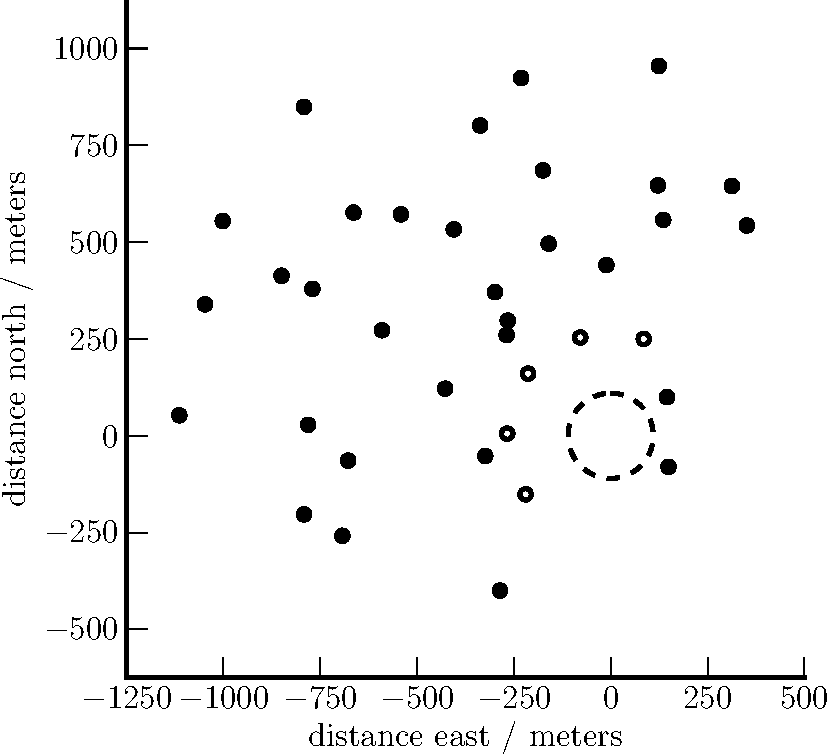
\includegraphics[width=\columnwidth]{plots/antenna-layout}
    \caption{
        This figure shows the antenna layout for the OVRO LWA.
        The 200 meter diameter area indicated by the dashed line contains 251 antennas distributed
        in a pseudo-random configuration. The 32 filled circles are the expansion antennas built in
        early 2016 to increase the longest baseline to 1.5 km. The 5 open circles are antennas
        equipped with noise-switched front ends.
    }
    \label{fig:antenna-layout}
\end{figure}

The Owens Valley Long Wavelength Array (OVRO LWA) is a 288-element interferometer located at the
Owens Valley Radio Observatory (OVRO) near Big Pine, California.  The OVRO LWA is a low-frequency
instrument with instantaneous bandwidth covering 24.768 MHz to 82.296 MHz \todo{double check this
frequency range, I think it's wrong}.  Each antenna stand hosts two perpendicular broadband dipoles
so that there are $288\times2$ signal paths in total. These signal paths feed into the 512-input
LEDA correlator, which allows the OVRO LWA to capture the entire visible hemisphere in a single
snapshot image.  In the current configuration, 32 antennas (64 signal paths) are unused.

The 288 antennas are arranged in a maximally non-redundant configuration optimized for minimum
sidelobes in snapshot imaging. 251 of these antennas are contained within a 200 m diameter core that
is independently optimized for imaging sidelobe levels. 32 antennas are placed outside of the core
in order to extend the maximum baseline length out to $\sim$1.5 km. The final 5 antennas are
equipped with noise-switched front ends for calibrated total power measurements of the global sky
brightness. These antennas are used as part of the LEDA experiment to measure the global signal of
21 cm absorption from the cosmic dawn. \todo{cite a leda paper} Calibrated total power measurements
from these antennas will be used to constrain sky modes with $l \lesssim 2$ including the monopole.
\todo{What values of $l$ actually contribute to the total power measurements?}

%See Figure~\ref{fig:antenna-layout} for an image of the antenna
%layout. The antennas can be categorized into 3 groups:
%\begin{enumerate}
%    \item
%        Core antennas - 251 antennas are contained within a 200 m diameter core where they are
%        arranged in a configuration optimized to reduce sidelobe levels in snapshot imaging.
%    \item
%        Total power antennas - 5 antennas are equipped with noise-switched front ends for calibrated
%        total power measurements of the sky brightness.
%    \item
%        Expansion antennas - 32 additional antennas were installed in early 2016. These antennas
%        extend the longest baselines of the OVRO LWA out to 1.5 km. This allows for $\sim10$
%        arcminute resolution in the snapshot images.
%\end{enumerate}
%When fully completed, the OVRO LWA will have 352 antennas in total spanning 2.5 km.
%
%\todo{cite Gregg's instrument paper}
%
%The field-of-view and compactness of the OVRO LWA make it a promising instrument for 21 cm
%cosmology. The field-of-view increases the number of cosmological modes measured at any instant in
%time. The inner core of 251 antennas within a 200 m diameter provides excellent brightness
%temperature sensitivity. Figure~\ref{fig:ps-sensitivity} shows the expected signal-noise ratio
%achieved by the OVRO LWA on the three-dimensional spatial power spectrum of 21 cm emission for a
%variety of models. A large integration time and careful calibration will be needed to make a
%detection.
%
%The Owens Valley Long Wavelength Array (OVRO LWA) is a 288-antenna interferometer located at the
%Owens Valley Radio Observatory (OVRO) near Big Pine, California. Each antenna is composed of two
%crossed dipoles bringing the total number of signal paths to 576.  The OVRO LWA hosts the LEDA
%correlator that allows cross-correlation of 512 signal paths with $>50$ MHz instantaneous bandwidth.
%
%Of the 288 antennas, 251 are located within a 200 m diameter core.  The location of these antennas
%has been optimized to minimize imaging sidelobes.  5 antenna stands are dedicated to the LEDA
%experiment and have switching front-ends for total-power radiometry. The remaining 32 antennas
%extend out to 2 km baselines to improve the angular resolution of the interferometer.

\subsection{The OVRO LWA 100 Hour Dataset}

Because the correlator only accepts 512 inputs (256 antennas with 2 polarizations for each antenna),
a subset of the antennas must be selected for correlation.

Include plot of antenna layout.

The integration time is 13 seconds. This was chosen because the remainder of one sidereal day
divided into 13 second intervals is only 90 milliseconds.  Finer control of the integration time is
not possible due to technical constraints.

\subsection{Antenna Gain Calibration}

Antenna gain calibration is accomplished using an iterative method independently developed by
\citet{2008ISTSP...2..707M} and \citet{2014A&A...571A..97S}. The calibration routine is written in
the Julia programming language \citep{BEKS14}, and is publicly available
online\footnote{\url{https://github.com/mweastwood/TTCal.jl}} under an open source license (GPLv3+).

The antenna complex gains are updated once per day from a 9 hour track of data when Cas A and Cyg A
are at high elevations.  These two sources are -- by an order of magnitude -- the brightest radio
sources in the northern hemisphere.  Therefore the optimal time to solve for the interferometer's
gain calibration is when Cas A and Cyg A are at high elevations. A calibration obtained in this
manner is good consistent with the following day's calibration to within a 1\% error in the flux
scale and 1$'$ error in the astrometry \todo{double check these numbers}. These residual errors are
likely driven by differing ionospheric conditions.

The flux scale is tied to the work of \citet{2016arXiv160905940P}.

\todo{sawtooth pattern removal, does it affect phase???}

\subsection{Source Removal}

\subsubsection{Cassiopeia A and Cygnus A}

Without removing bright sources from the data, sidelobes from bright sources will dominate the
variance in the image.  At 74 MHz Cyg A is a 15,000 Jy source \citep{2016arXiv160905940P}. A
conservative estimate for the confusion limit at 74 MHz with a 10 arcminute beam is 500 mJy
\citep{2012RaSc...47.0K04L}. Therefore we require that Cyg A's sidelobes be at most of $-$45 dB down
from its peak flux to prevent Cyg A's sidelobes from dominating the variance in the image.
\todo{Measure Cyg A's sidelobe levels if it is not subtracted}

At low frequencies, propagation effects through the ionosphere must be accounted for in order to
achieve high dynamic range images. This necessitates the use of direction-dependent calibration and
peeling \citep{2008ISTSP...2..707M, 2015MNRAS.449.2668S}.  In the dataset used in this paper,
scintillation and diffraction events on the timescale of a single integration (13 seconds) are
observed. Therefore the direction dependent calibration changes on these timescales and the we must
solve for one set of complex gains per source per integration.

The largest angular scale of Cas A is $\sim$8 arcminutes, while the largest angular scale of Cyg A
is $\sim$2 arcminutes. With a 10 arcminute resolution, the OVRO LWA marginally resolves both
sources. A resolved source model is needed for both sources. We fit a self-consistent resolved
source model to eachs ource. This is performed by minimizing the minimizing the variance within an
aperture located on each source after peeling. By phasing up a large number of integrations before
imaging (at least over 1 hour) it is possible to smear out the contribution of the rest of the sky.
We then use NLopt's Sbplx routine \citep{nlopt, sbplx} to vary the parameters in a source model
until the variance within the aperture is minimized.

\todo{Show a before and after with the updated source models}

\todo{Give a plot with the updated source models}

\subsubsection{The Sun}

The Sun can be trivially removed from any map of the sky by constructing the map using only data
taken at night. A map of the entire sky can be obtained by using observations spaced 6 months apart.
However the OVRO LWA 100 hour dataset consists of 100 consecutive hours of data, and hence roughly
half of the data is from the day.

The Sun is a time variable source in radio.

\todo{does the previous routine work on the Sun too? worth a shot}

\subsubsection{Sparking Power Lines}

The Owens Valley is an important source of water and power for the city of Los Angeles.
Unfortunately this means that high voltage power lines run along the valley to the west of the OVRO
LWA. Some of these power line poles have faulty insulators that arc and produce pulsed, broadband
RFI. Because these poles exist in the near-field of the array, we have been able to localize some of
them by using the curvature of the incoming wavefront. Efforts are currently underway to work with
the utility pole owners to have these insulators replaced.

In the meantime it is possible to suppress their contamination in the dataset. The contribution of
these RFI sources to the visibilities can be plainly seen by averaging $>$24 hours of data with the
phase center set to zenith. In this way, true sky components are smeared along tracks of constant
declination while terrestrial sources (ie. the arcing power lines) are not smeared. For similar
reasons, when constructing a map of the sky from $>$24 hours of data these sparking power lines will
produce artifacts in the map that are smeared along tracks of constant declination. However while
the amplitude of the RFI will fluctuate with time, its phase will be constant. Therefore if you can
use isolate a set of model visibilities for the RFI, it can be removed from each integration by
scaling and subtracting these model visibilities from the measured visibilities.

Obtaining a model for the RFI is complicated by the fact that the contaminating sources are at
extremely low elevations where the antenna response is maximally inhomogeneous. Therefore it is not
enough to know the physical location of the faulty insulator generating the RFI. In addition you
must also know the response of each antenna (amplitude and phase) in the appropriate direction. This
motivates the use of peeling, which allows the antenna response to be a free parameter.

Therefore model visibilities for the RFI can be obtained by peeling the sources after smearing the
visibilities over $>$24 hours. These model visibilities are then scaled and subtracted from each
integration in the data set.

\todo{show an example smeared image before and after peeling}

\subsection{Fitting the Antenna Response}

In order to generate wide-field images of the sky, the response of the antenna to the sky must be
known. Fortunately drift-scanning interferometers like the OVRO LWA can empirically measure their
primary beam under a mild set of symmetry assumptions \citep{2012AJ....143...53P}. In this work we
assume that the primary beam is invariant under north-south and east-west flips, and additionally
that the $x$- and $y$-dipoles have the same response to the sky after rotating one by 90$^\circ$.
We measure the flux of several point sources \todo{which ones??} as they pass through the sky and
then fit a beam model composed of Zernike polynomials to those flux measurements. We select the
basis functions to have the desired symmetry.

\section{Imaging}

The goal of all imaging algorithms is to estimate the brightness of the sky $I_\nu(\hat r)$ in the
direction $\hat r$ and frequency $\nu$. A radio interferometer measures the visibilities
$V_{ij,\nu}$ between pairs of antennas -- here numbered $i$ and $j$ respectively. If the antennas
are separated by the baseline $\vec b_{ij}$, and $A_\nu(\hat r)$ describes their response to the
incident radiation, then
\begin{equation}\label{eq:basic-imaging}
    V^{ij}_\nu = \int_\text{sky}
                 A_\nu(\hat r) I_\nu(\hat r)
                 \exp\bigg(2\pi i \hat r\cdot\vec b_{ij}/\lambda\bigg) \,\d\Omega \, .
\end{equation}
Imaging the output of a radio interferometer therefore consists of estimating $I_\nu(\hat r)$ given
the available measurements $V^{ij}_\nu$.

Naively one might attempt to solve equation~\ref{eq:basic-imaging} by discretizing, and subsequently
solving the resulting matrix equation. If the interferometer is composed of $N_\text{base}$
baselines, and measures $N_\text{freq}$ frequency channels over $N_\text{time}$ integrations then
the entire data set consists of $N_\text{base}N_\text{freq}N_\text{time}$ complex numbers. If the
sky is discretized into $N_\text{pix}$ pixels then the relevant matrix has dimensions of
$(N_\text{base}N_\text{freq}N_\text{time})\times(N_\text{pix})$. For making single-channel maps with
the Owens Valley LWA this becomes a 5 petabyte array (assuming each matrix element is a 64-bit
complex floating point number).  This matrix equation is therefore prohibitively large, and solving
equation~\ref{eq:basic-imaging} by means of discretization is usually impossible \todo{cite Jayce's
paper (has he published that yet?) where he does this, but explain why his work is the exception
instead of the rule}.

Instead it is common to make mild assumptions that simplify equation~\ref{eq:basic-imaging} and ease
the computational burden in solving for $I_\nu(\hat r)$. For example, when all of the baselines
$\vec b_{ij}$ lie in a plane and the field-of-view is small, equation~\ref{eq:basic-imaging} can be
well-approximated by a two-dimensional Fourier transform.

\todo{discuss w-projection}

\todo{discuss a-projection}

\citet{2017MNRAS.465.2901Z}

\subsection{$m$-Mode Analysis}

On the other hand, transit telescopes can take advantage of a symmetry in
equation~\ref{eq:basic-imaging} that greatly reduces the amount of computer time required to image
the full-sky with exact incorporation of widefield imaging effects. This technique, called $m$-mode
analysis, also obviates the need for gridding, mosaicing, and multi-scale deconvolution. Instead the
entire sky is imaged in one coherent synthesis imaging step.

In this context we will define a transit telescope as any interferometer where the response pattern
of the individual elements does not change with respect to time. This may be an interferometer like
the OVRO LWA where the correlation elements are fixed dipoles, but it may also be an interferometer
like the MWA if the steerable beams are held in a fixed position (not necessarily at zenith).

We will briefly summarize $m$-mode analysis below, but the interested reader should consult
\citet{2014ApJ...781...57S, 2015PhRvD..91h3514S} for a complete derivation.

For a transit telescope, the visibilities $V^{ij}_\nu$ are a periodic function of sidereal
time\footnote{
    This is not strictly true. Ionospheric fluctuations and non-sidereal sources (such as the sun)
    will violate this assumption. This paper will, however, demonstrate that the impact on the final
    maps is mild.
}.
Therefore it is a very natural operation to compute the Fourier transform of the visibilities with
respect to sidereal time $\phi\in(0,2\pi]$.
\begin{equation}
    V^{ij}_{m,\nu} = \int_0^{2\pi} V^{ij}_\nu(\phi)\exp\bigg(-im\phi\bigg)\,\d\phi
\end{equation}
The output of this Fourier transform is the set of $m$-modes $V^{ij}_{m,\nu}$ where
$m=0,\,\pm1,\,\pm2,\,\ldots$ is the Fourier conjugate variable to the sidereal time. The $m$-mode
corresponding to $m=0$ is a simple average of the visibilities over sidereal time. Similarly $m=1$
corresponds to the component of the visibilities that varies over half-day timescales. Larger values
of $m$ correspond to components that vary on quicker timescales.

\todo{introduce the baseline transfer function because I will want to use it in later sections}

It can be shown that there is a discrete linear relationship between the $m$-modes $V^{ij}_{m,\nu}$
and the spherical harmonic coefficients of the sky brightness $a_{lm,\nu}$.
\begin{equation}\label{eq:m-mode-sum-equation}
    V^{ij}_{m,\nu} = \sum_l B^{ij}_{lm,\nu} a_{lm,\nu}\,,
\end{equation}
where the transfer coefficients $B^{ij}_{lm,\nu}$ define the interferometer's response to the sky.
For example, the transfer coefficients are a function of the baseline and antenna primary beam
pattern.

Equation~\ref{eq:m-mode-sum-equation} can be recognized as a matrix equation where the transfer
matrix $\b B$ is block-diagonal.
\begin{equation}
    \b B = \left(\begin{array}{cccc}
        m = 0 &&& \\
              & m=\pm1 && \\
              && m=\pm2 & \\
              &&& \ddots \\
    \end{array}\right)
\end{equation}
The vector $\b v$ contains the list of $m$-modes and the vector $\b a$ contains the list of
spherical harmonic coefficients representing the sky brightness. In order to take advantage of the
block-diagonal structure in $\b B$, $\b v$ and $\b a$ must be sorted by the value of $m$.
\begin{equation}\label{eq:m-mode-matrix-equation}
    \overbrace{\left(
        \begin{array}{c}
            \vdots \\
            m\text{-modes} \\
            \vdots \\
        \end{array}
    \right)}^{\b v}
    =
    \overbrace{\left(
        \begin{array}{ccc}
            \ddots & & \\
            & \text{transfer matrix} & \\
            & & \ddots \\
        \end{array}
    \right)}^{\b B}
    \overbrace{\left(
        \begin{array}{c}
            \vdots \\
            a_{lm} \\
            \vdots \\
        \end{array}
    \right)}^{\b a}
\end{equation}

In practice we now need to pick the set of spherical harmonics we will use to represent the sky. For
an interferometer like the OVRO LWA with lots of short baselines, a sensible choice is to use all
spherical harmonics with $l\le l_\text{max}$ for some $l_\text{max}$. The parameter $l_\text{max}$
is determined by the maximum baseline length of the interferometer.  For an interferometer without
short spacings, a minimum value for $l$ might also be used. This $l_\text{min}$ parameter should be
determined by the minimum baseline length.  When creating the maps presented in this paper, we use
$l_\text{min} = 0$ and $l_\text{max} = 1000$.
\todo{exclude l = 0 and cite tejas' paper}

The size of a typical block in the transfer matrix is
$(2N_\text{base}N_\text{freq})\times(l_\text{max})$. If each element of the matrix is stored as a
64-bit complex floating point number, a single block is 500 MB for the case of single-channel
imaging with the OVRO LWA. Compare this number with the 5 PB required for the naive approach.  The
power of $m$-mode analysis is the block-diagonal structure of
equation~\ref{eq:m-mode-matrix-equation}.  By breaking up the problem into $N$ independent blocks,
the computational complexity involved in inverting the equation is reduced by a factor $N^3$. For
the case of the OVRO LWA the equation breaks up into $\sim10^3$ blocks and so we save a factor of
$\sim10^9$ in processing time by using $m$-mode analysis.

Imaging in $m$-mode analysis essentially amounts to inverting
equation~\ref{eq:m-mode-matrix-equation} to solve for the spherical harmonic coefficients $\b a$.
The linear-least squares solution, which minimizes $\|\b v - \b B\b a\|^2$, is given by
\begin{equation}
    \b{\hat a}_\text{LLS} = (\b B^*\b B)^{-1}\b B^*\b v\,,
\end{equation}
where $^*$ indicates the conjugate-transpose. However, usually one will find that $\b B$ is not
full-rank and hence $\b B^*\b B$ is not an invertible matrix. For example, an interferometer located
in the northern hemisphere will never see a region of the southern sky centered on the southern
celestial pole. The $m$-modes contained in the vector $\b v$ must contain no information
about the sky around the southern celestial pole, and therefore the act of multiplying by $\b B$
must destroy some information about the sky. The consequence of this fact is that $\b B^*\b B$ must
have at least one zero eigenvalue, which means it is not invertible.

Another way of looking at the problem is that because the interferometer is not sensitive to part of
the southern hemisphere, there are infinitely many possible solutions to
equation~\ref{eq:m-mode-matrix-equation} that will fit the measured data equally well. So we need to
regularize the problem and apply an additional constraint that prefers a unique solution. For
example, you may prefer that in the absence of any information the sky should be set to zero or you
may prefer that the sky should be set to some prior expectation. The process of Tikhonov
regularization minimizes $\|\b v - \b B\b a\|^2 + \epsilon\|\b a\|^2$ for some arbitrary value of
$\epsilon > 0$ chosen by the observer. The solution that minimizes this expression is given by
\begin{equation}
    \b{\hat a}_\text{Tikhonov} = (\b B^*\b B + \epsilon\b I)^{-1}\b B^*\b v\,.
\end{equation}
Tikhonov regularization adds a small value $\epsilon$ to the diagonal of $\b B^*\b B$, fixing the
matrix's singularity.

\todo{describe how Tikhonov regularization improves the noise properties of the map}

\todo{describe the Moore-Penrose pseudoinverse and why I have elected not to use it}

While Tikhonov regularization will force unmeasured modes to zero, if a prior map of the sky already
exists, it will be preferrable to instead minimize $\|\b v - \b B\b a\|^2 + \epsilon \|\b a-\b
a_\text{prior}\|^2$.

Tikhonov regularization requires the observer to pick the value of $\epsilon$. If $\epsilon$ is too
large then too much importance is placed on minimizing the norm of the solution and the
least-squares residuals will suffer. However if $\epsilon$ is too small then the problem will be
poorly regularized and the resulting sky map may not represent the true sky.

A tool that can be used to address this problem is the L-Curve.

\subsection{$m$-Mode Analysis with the OVRO LWA}






\subsection{CLEAN}

\section{Errors}

\subsection{Stationary Correlated Noise}

However it is instructive to analyze the contaminating effect the RFI will have
on $m$-mode analysis maps of the sky. The correlation observed on a given
baseline and frequency channel for a single source of RFI is
\begin{equation}
    V(t) = I(t) B^\textrm{near-field}
\end{equation}

However we need a strategy to mitigate the RFI before imaging. A constant source attached to the
horizon has a fringe rate of zero. The only possible astronomical origins for a source with zero
fringe rate are:

\begin{enumerate}
    \item a point source located at the north or south celestial poles, and
    \item a ring of constant declination.
\end{enumerate}

Therefore while snapshot images will show the RFI source on the horizon, extended integrations will
show the RFI as rings of constant declination. We can take advantage of this discrepancy to separate
astronomical emission from terrestrial RFI.




\subsection{Ionospheric Scintillation}

One of the key assumptions made by $m$-mode analysis is that the sky is completely static.  We
assume that the only time-dependent behavior is the rotation of the Earth, which slowly rotates the
sky through the fringe patterns of the interferometer. At low frequencies the ionosphere violates
this assumption. In particular, ionospheric scintillation will cause even static sources to exhibit
significant variability.

The correlation observed on a given baseline for a single point source is
\begin{equation}
    V_\nu(t_{\textrm{sidereal}}) = I_\nu B_\nu(t_{\textrm{sidereal}}),
\end{equation}
where $I_\nu$ is the flux of the source at the frequency $\nu$, and $B_\nu$
is the baseline transfer function. The transfer function is a function of
the direction to the source, which is in turn a function of the sidereal
time $t_{\textrm{sidereal}}$. If the source is varying, from intrinsic
variability or due to scintillation, than the source flux is also a function
of the time coordinate $t$ such that
\begin{equation}
    V_\nu(t_{\textrm{sidereal}}) = I_\nu(t) B_\nu(t_{\textrm{sidereal}}),
\end{equation}
where $t_{\textrm{sidereal}} = (t \mod 23.9345\,\textrm{hours})$.

Now assume we have observed with our interferometer for a single sidereal day.
In order to compute the $m$-modes we must Fourier transform with respect to
sidereal time. In a real measurement this is a discrete Fourier transform of
the observed correlation with respect to time (where the sum over time is
restricted to a sidereal day). \todo{fix normalization}
\begin{equation}
    V_{\nu, m} = \sum_{t} V_\nu(t) e^{-imt}
\end{equation}
Define $V_{\nu, m}^{\textrm{static}}$ to be the observed $m$-modes if the source
was actually static ($I_\nu(t) \equiv I_{\nu,0}$). Then as a consequence of the
Fourier convolution theorem
\begin{equation}
    V_{\nu, m} = \sum_{m^\prime} V_{m^\prime}^\textrm{static} I_{\nu, m-m^\prime}.
\end{equation}

This will tend to scatter power between $m$-modes.

Simulate images of point sources with this


\subsection{Ionospheric Refraction}


\subsection{Beam Errors}


\section{Results}

\subsection{Sky Maps}

\begin{figure*}[ht]
    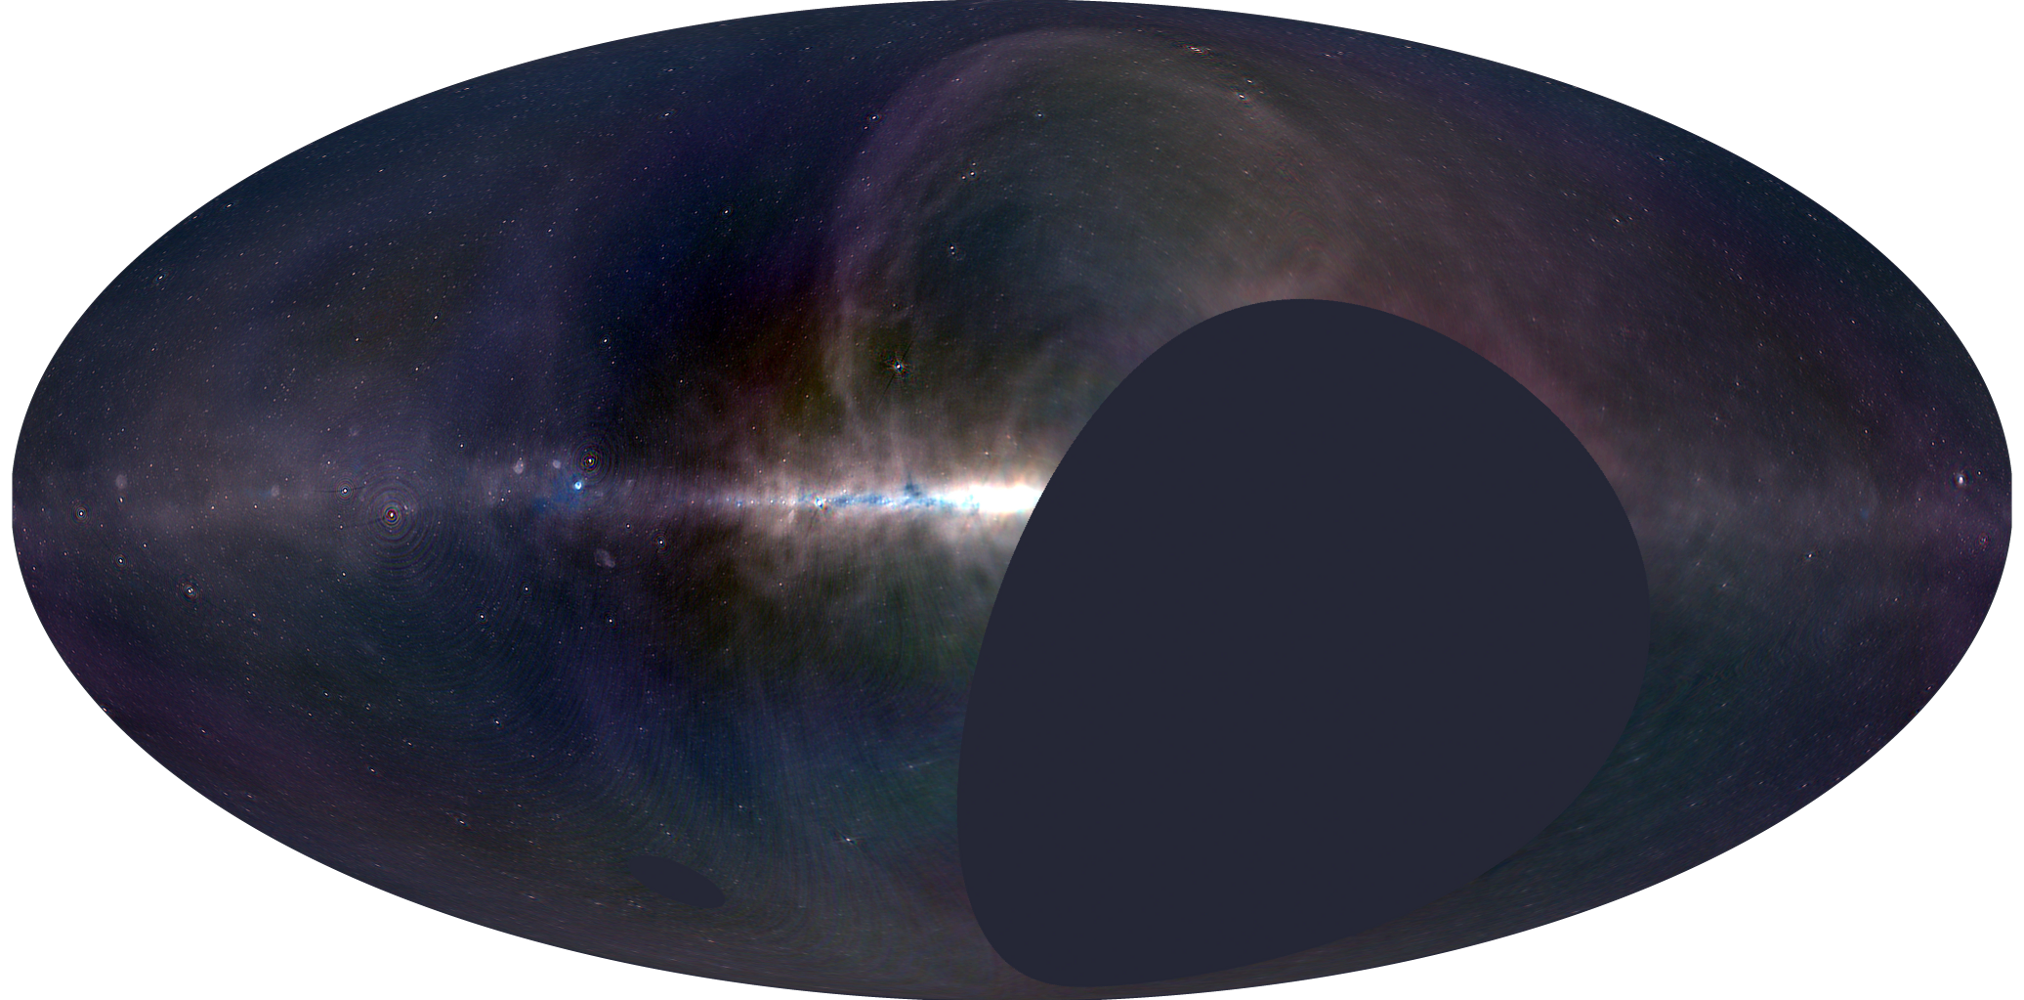
\includegraphics[width=\textwidth, draft]{maps/rgb-map}
    \caption{three color map}
\end{figure*}

\begin{figure*}[ht]
    \centering
    \begin{tabular}{cc}
        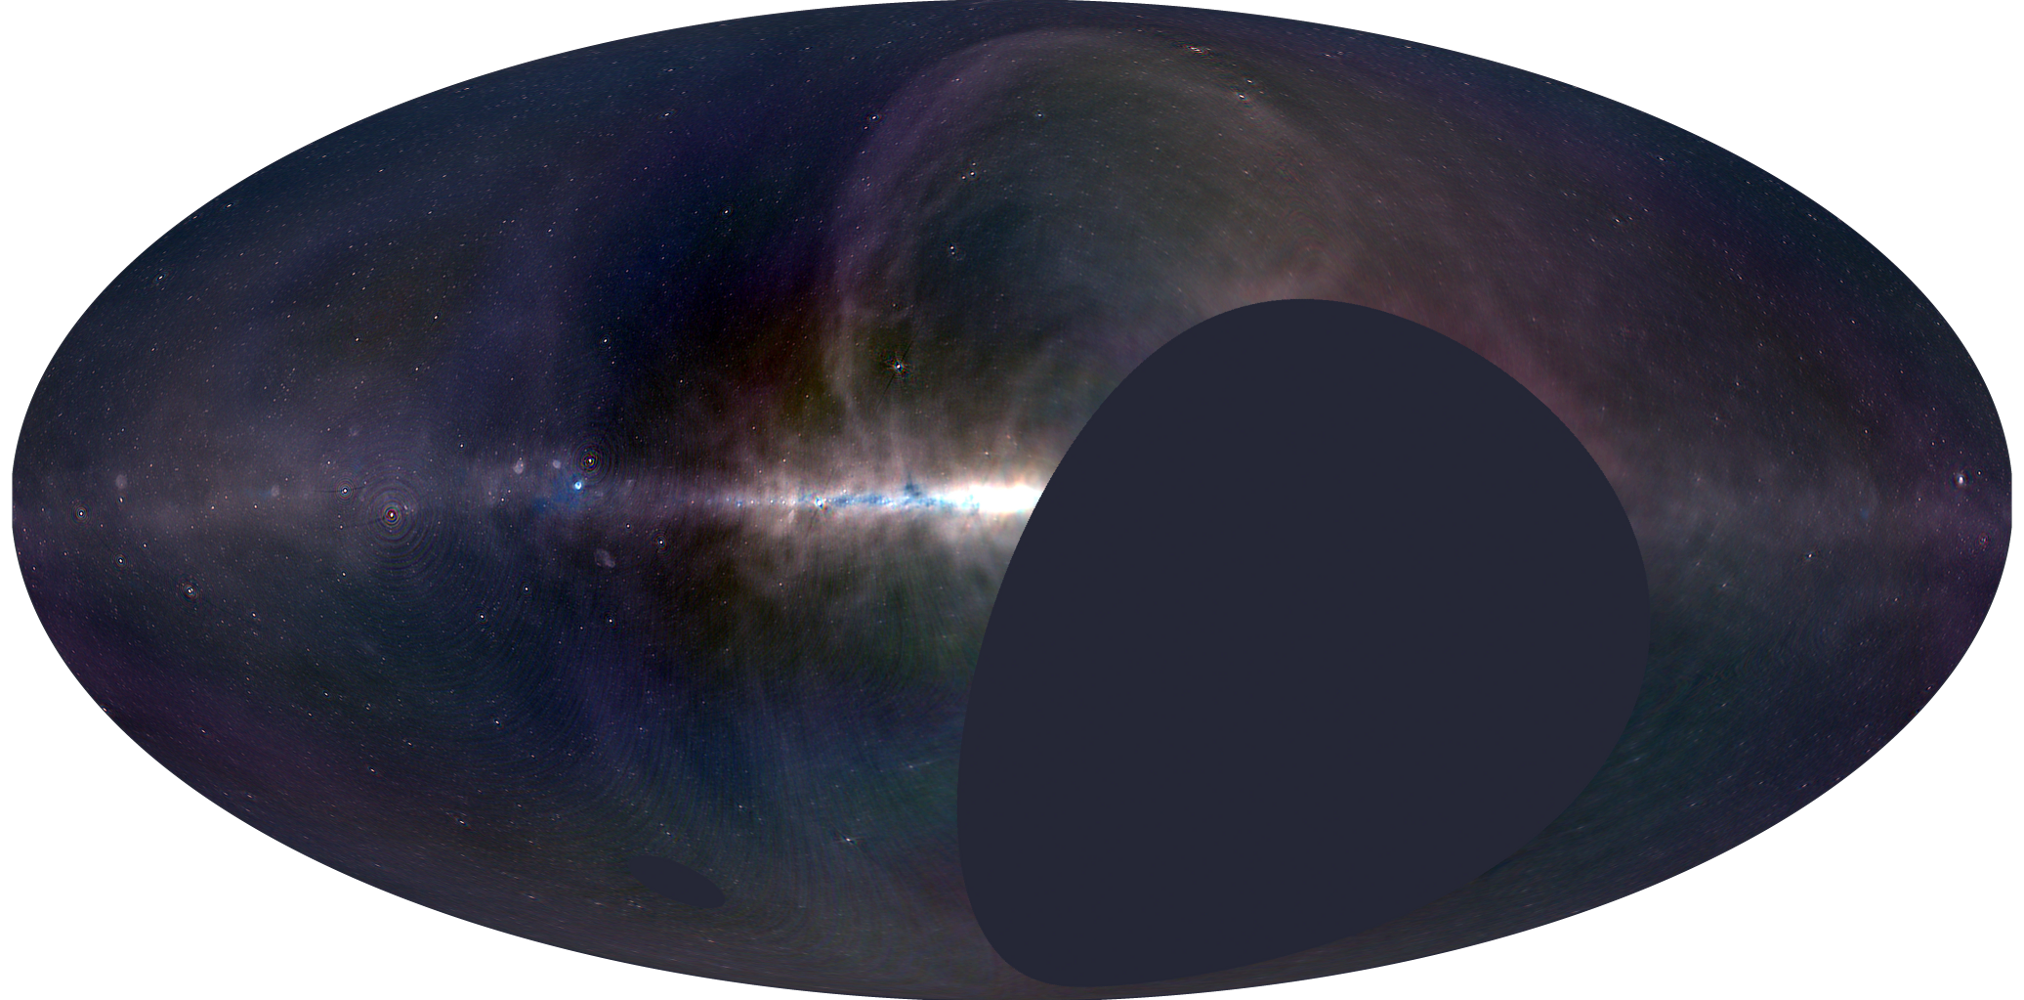
\includegraphics[width=\columnwidth, draft]{maps/rgb-map} &
        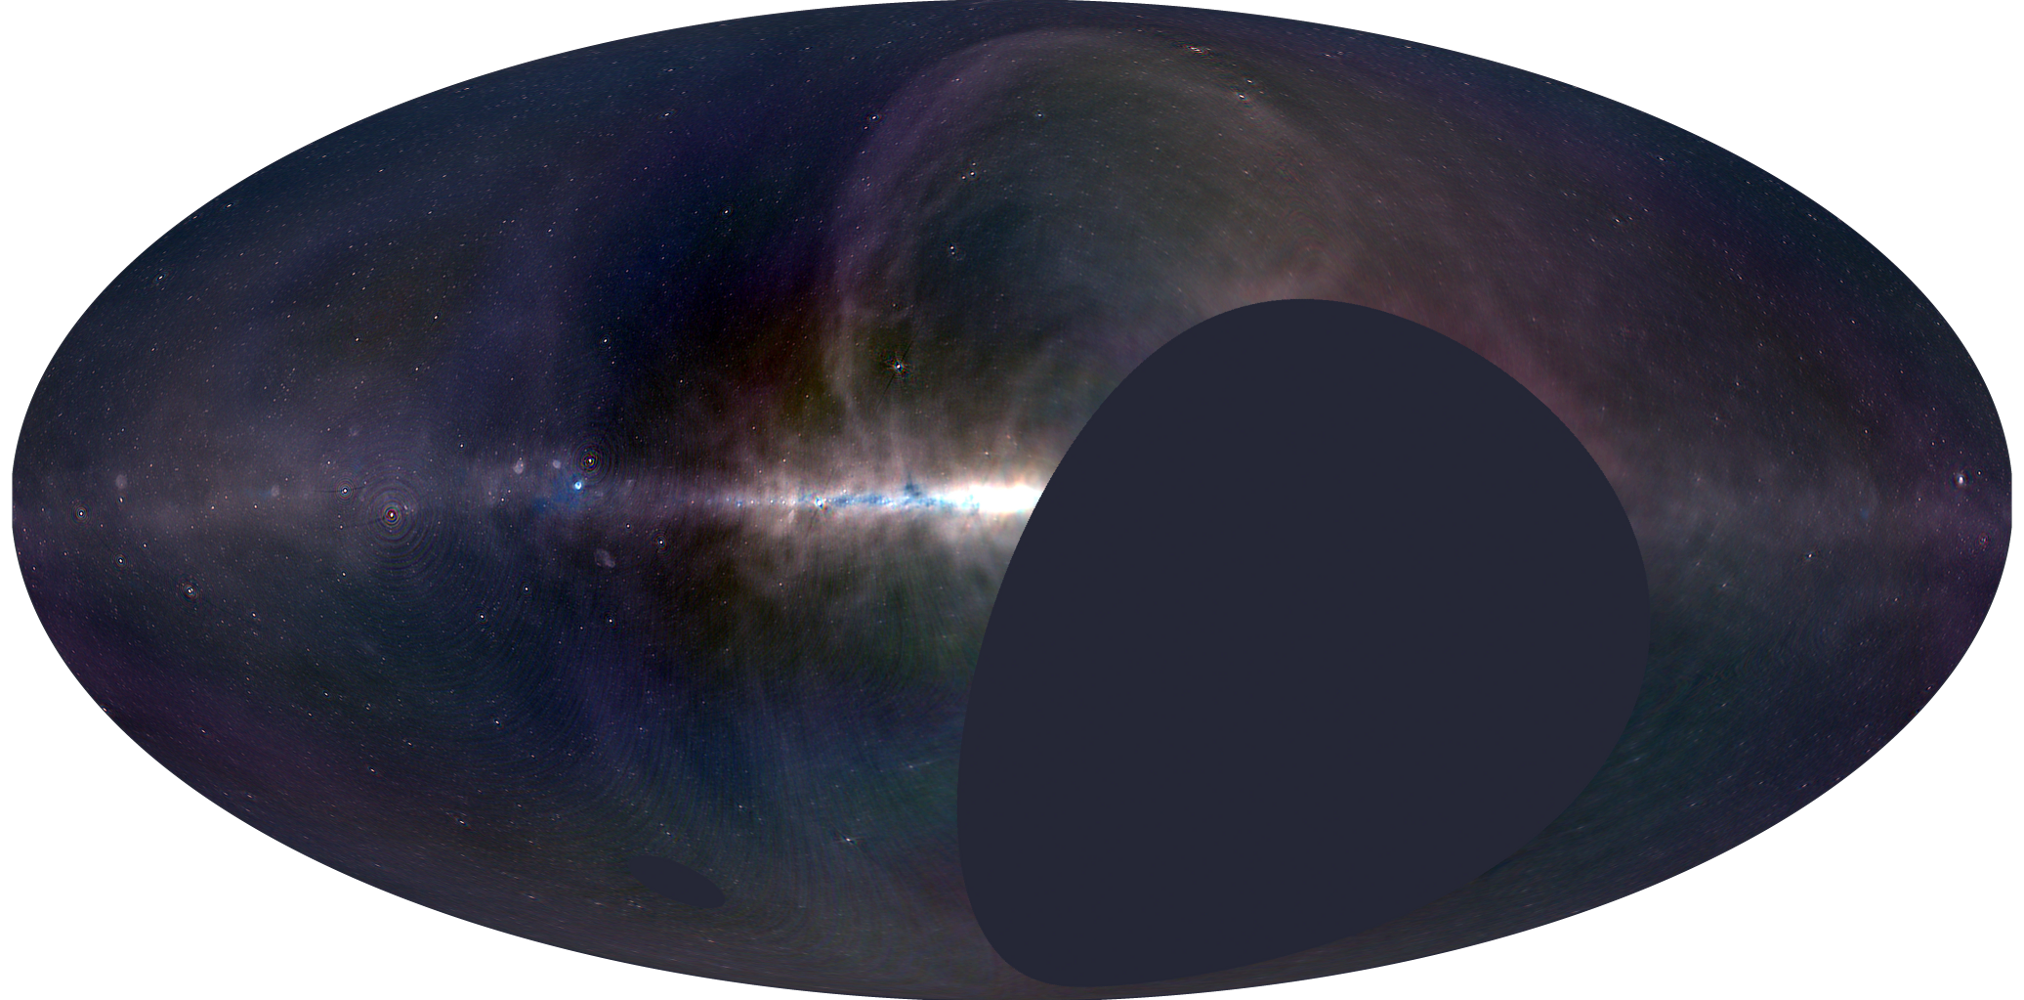
\includegraphics[width=\columnwidth, draft]{maps/rgb-map} \\
        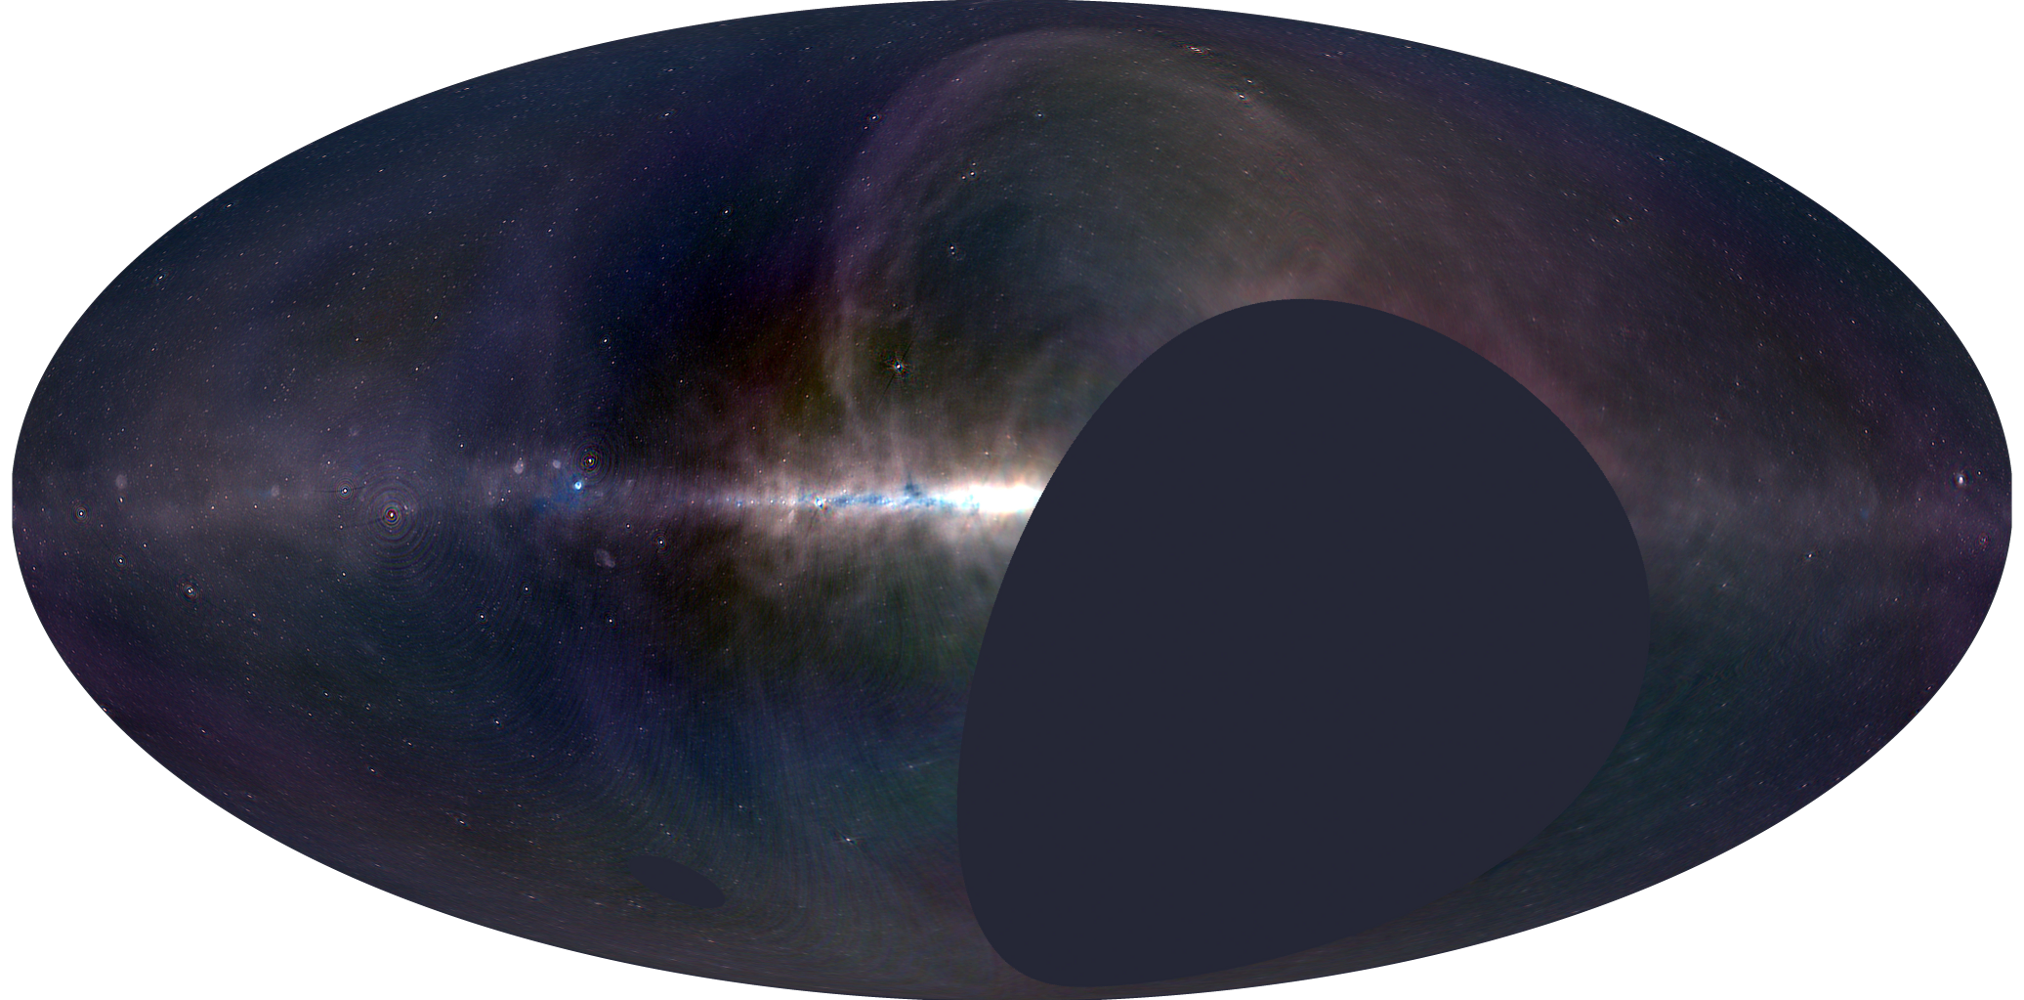
\includegraphics[width=\columnwidth, draft]{maps/rgb-map} &
        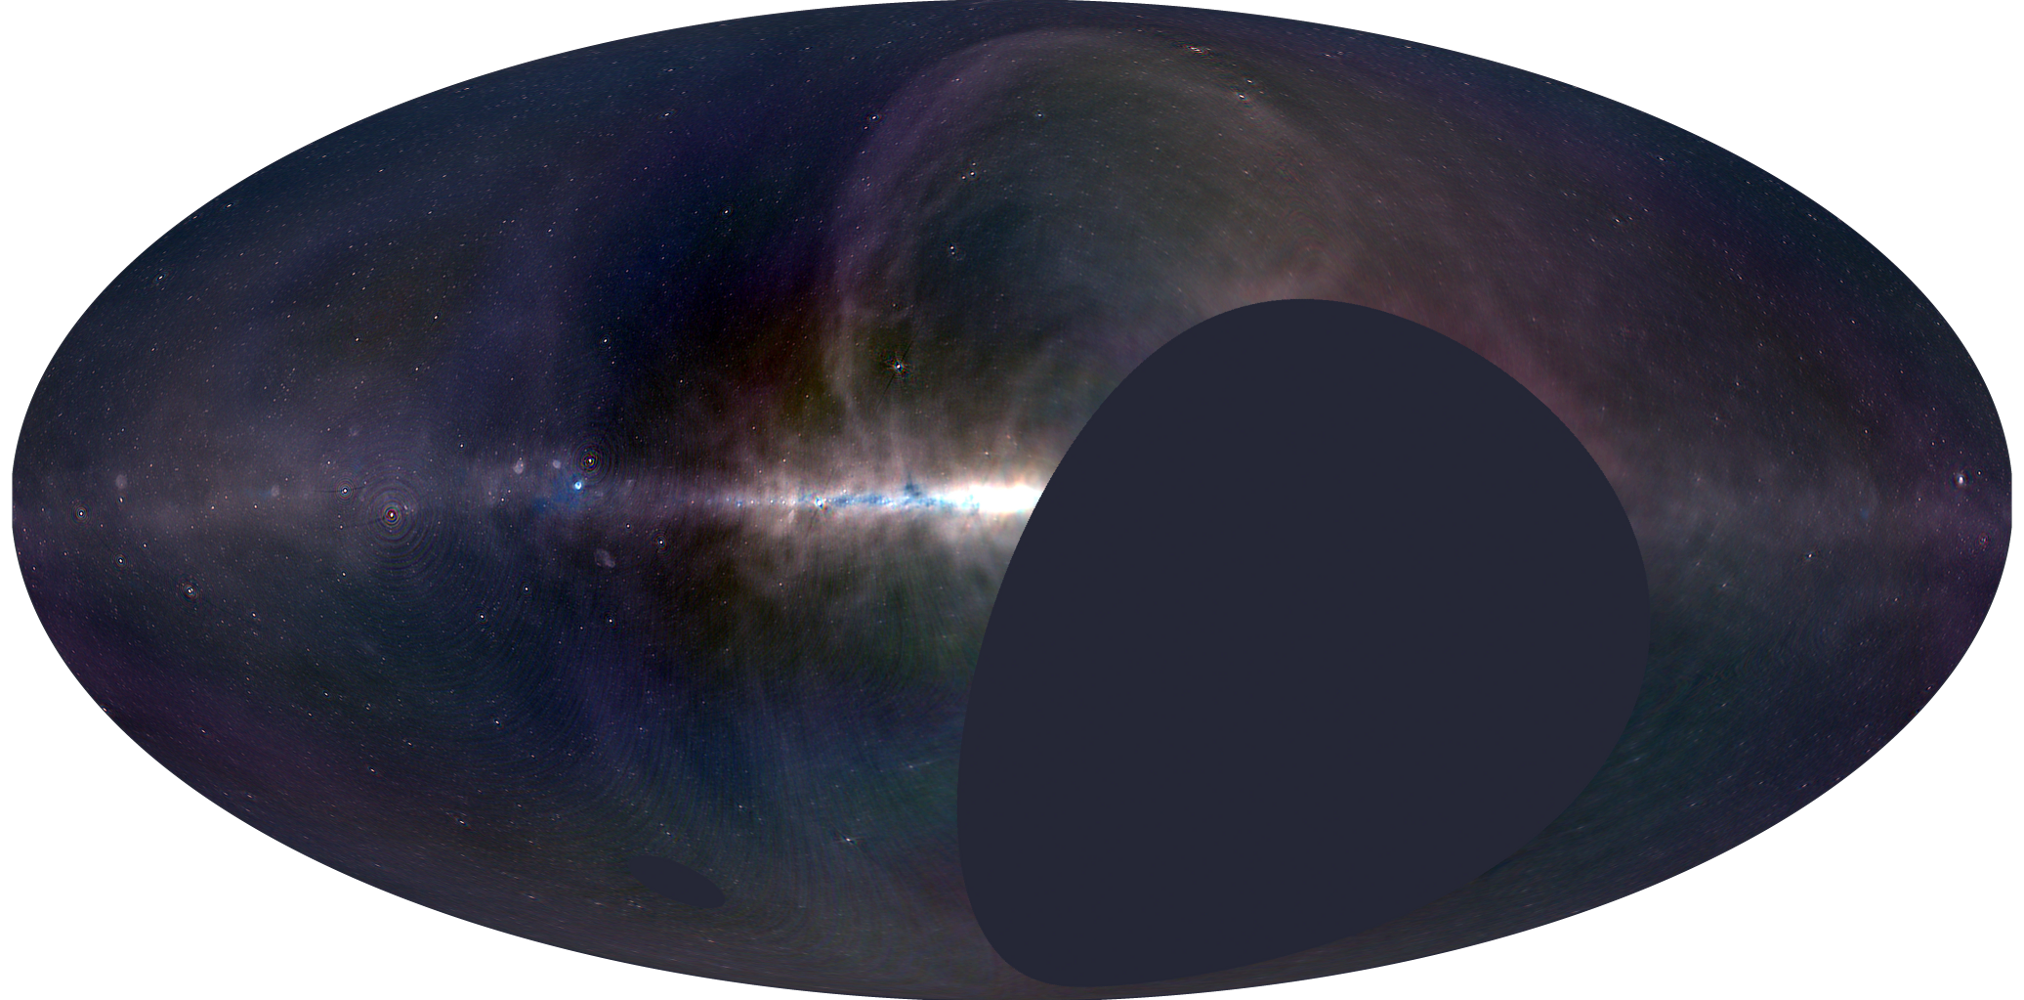
\includegraphics[width=\columnwidth, draft]{maps/rgb-map} \\
        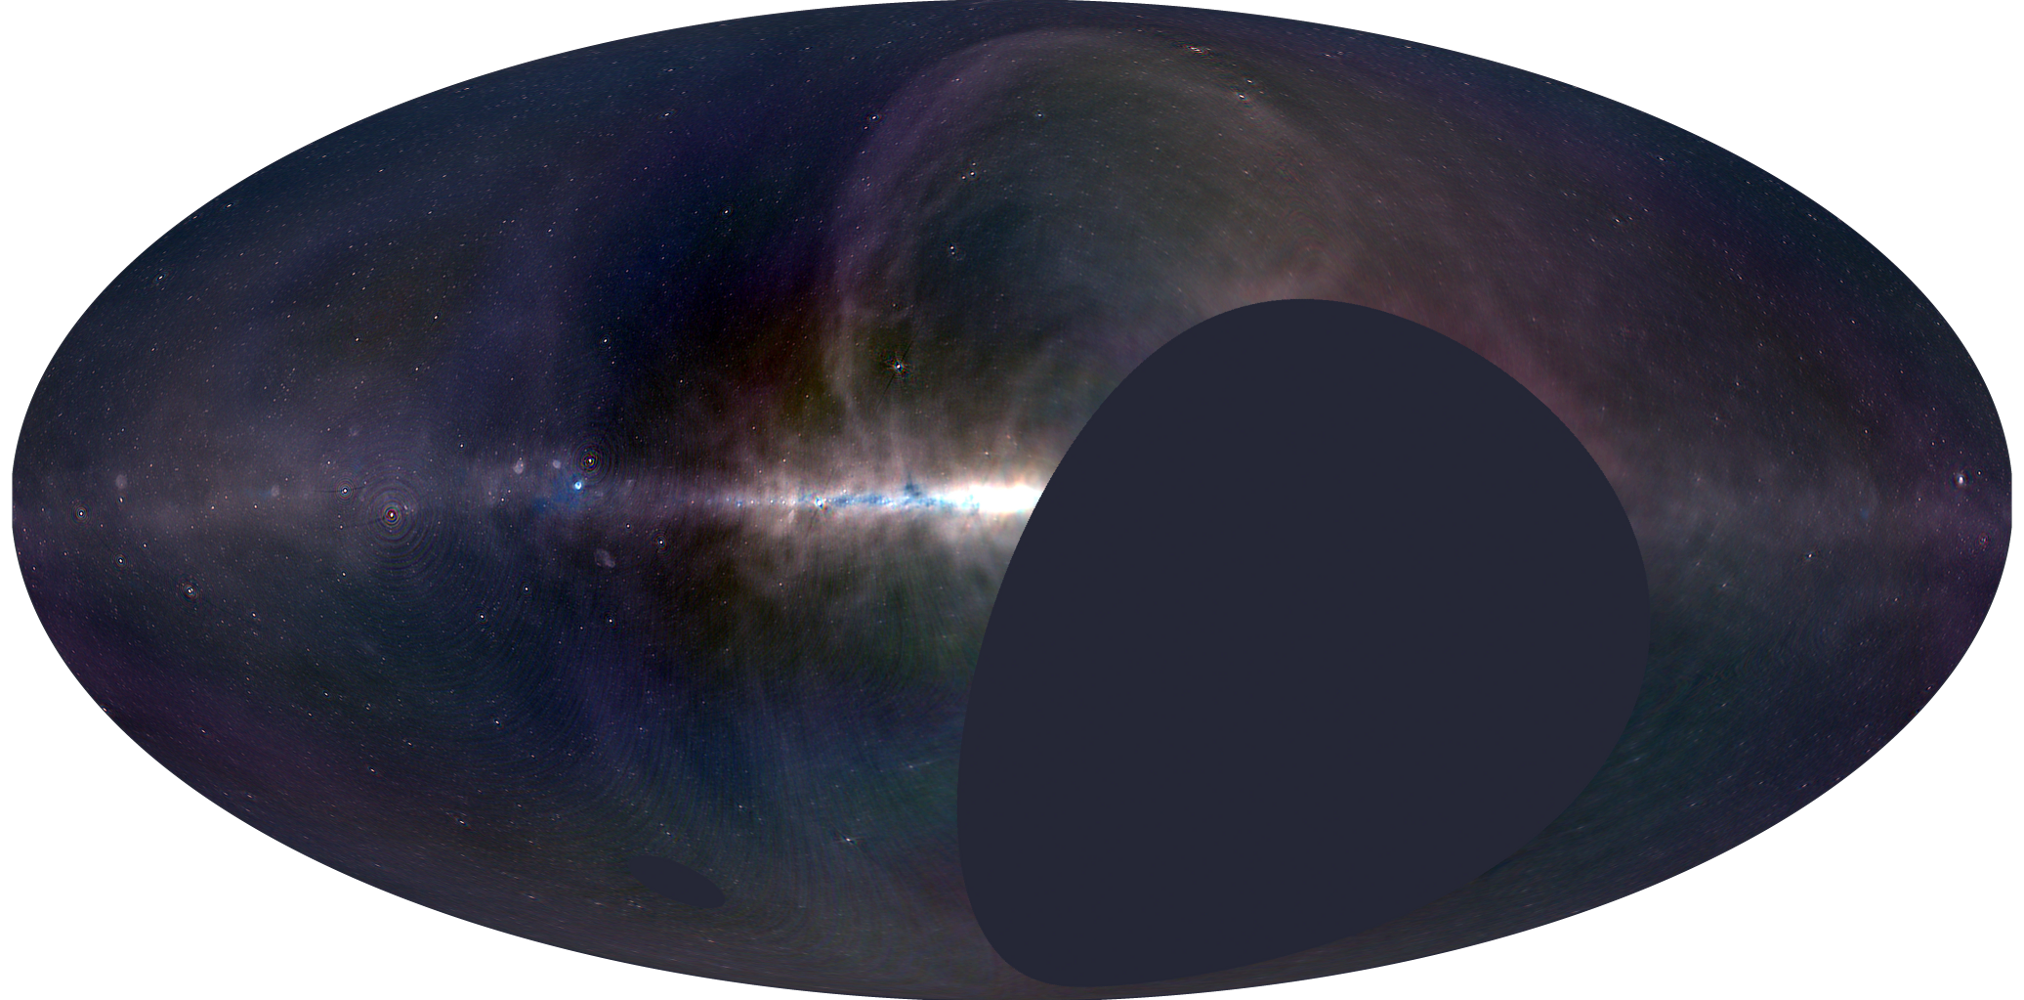
\includegraphics[width=\columnwidth, draft]{maps/rgb-map} &
        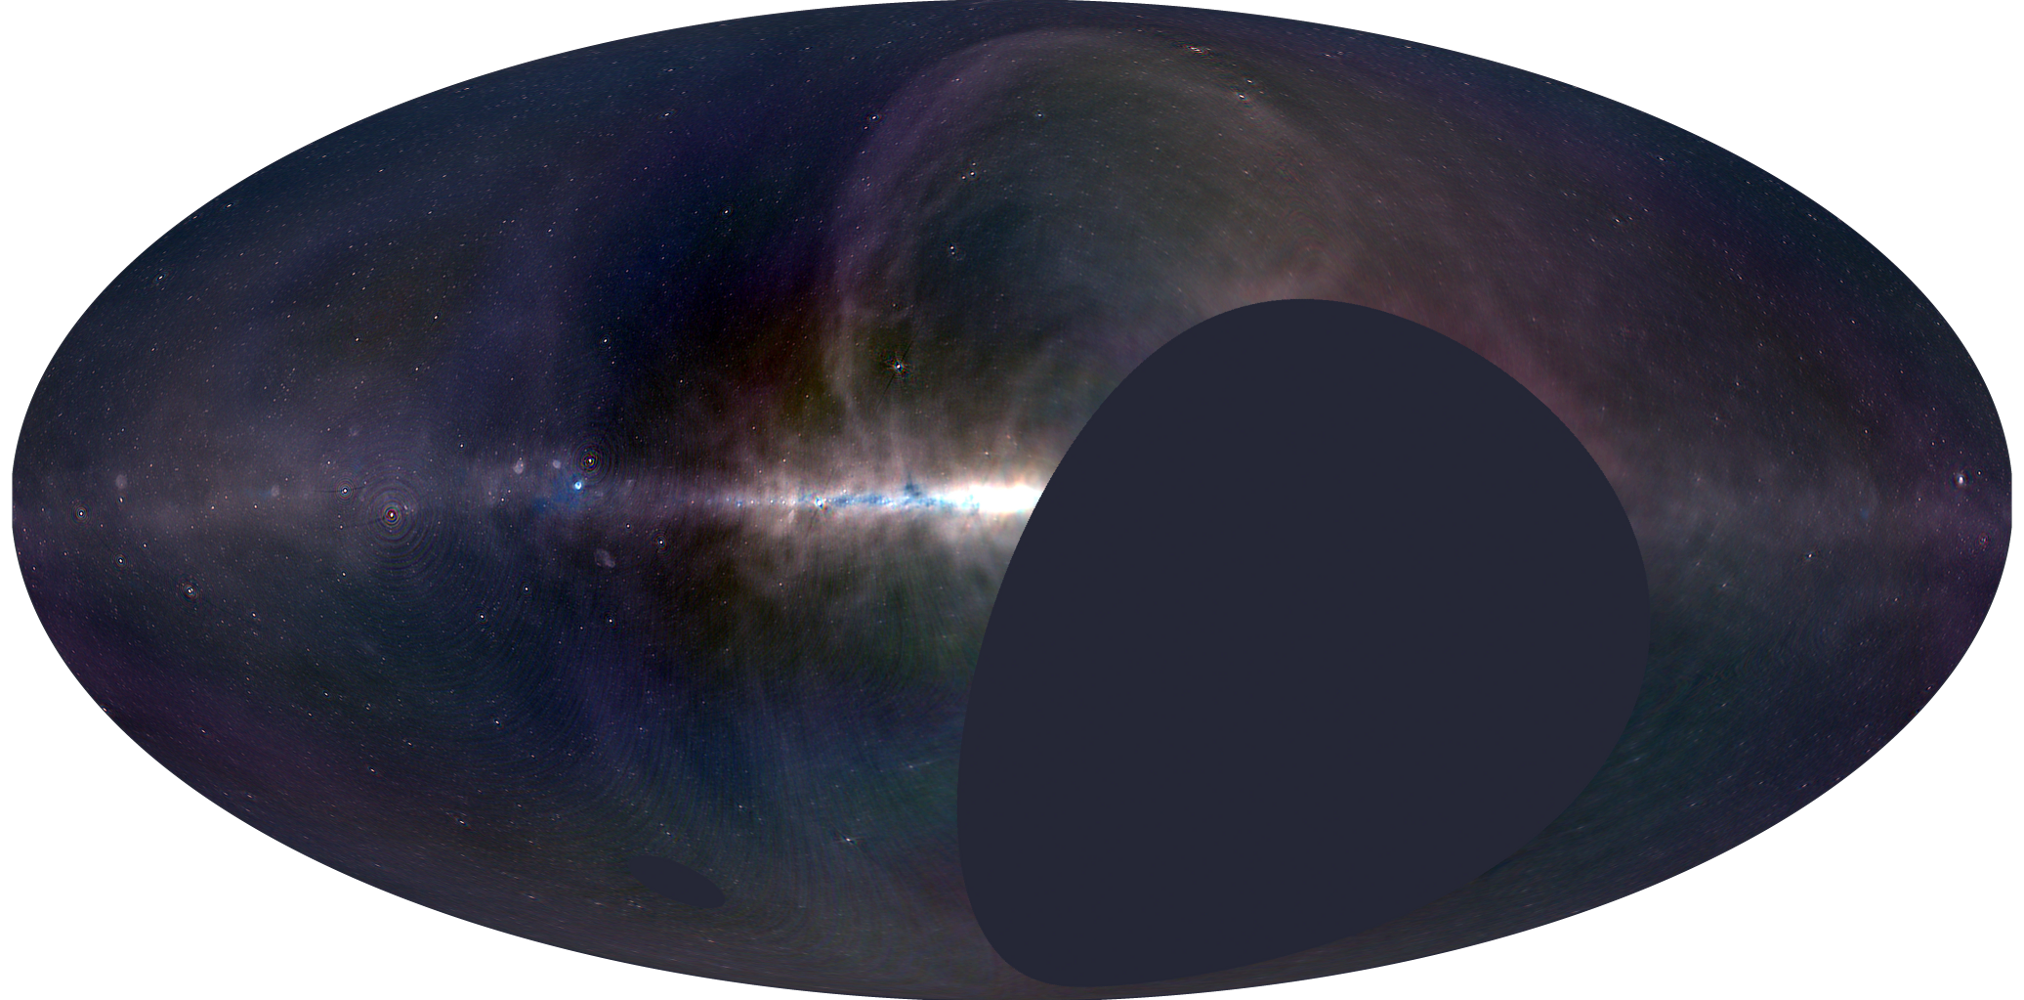
\includegraphics[width=\columnwidth, draft]{maps/rgb-map} \\
        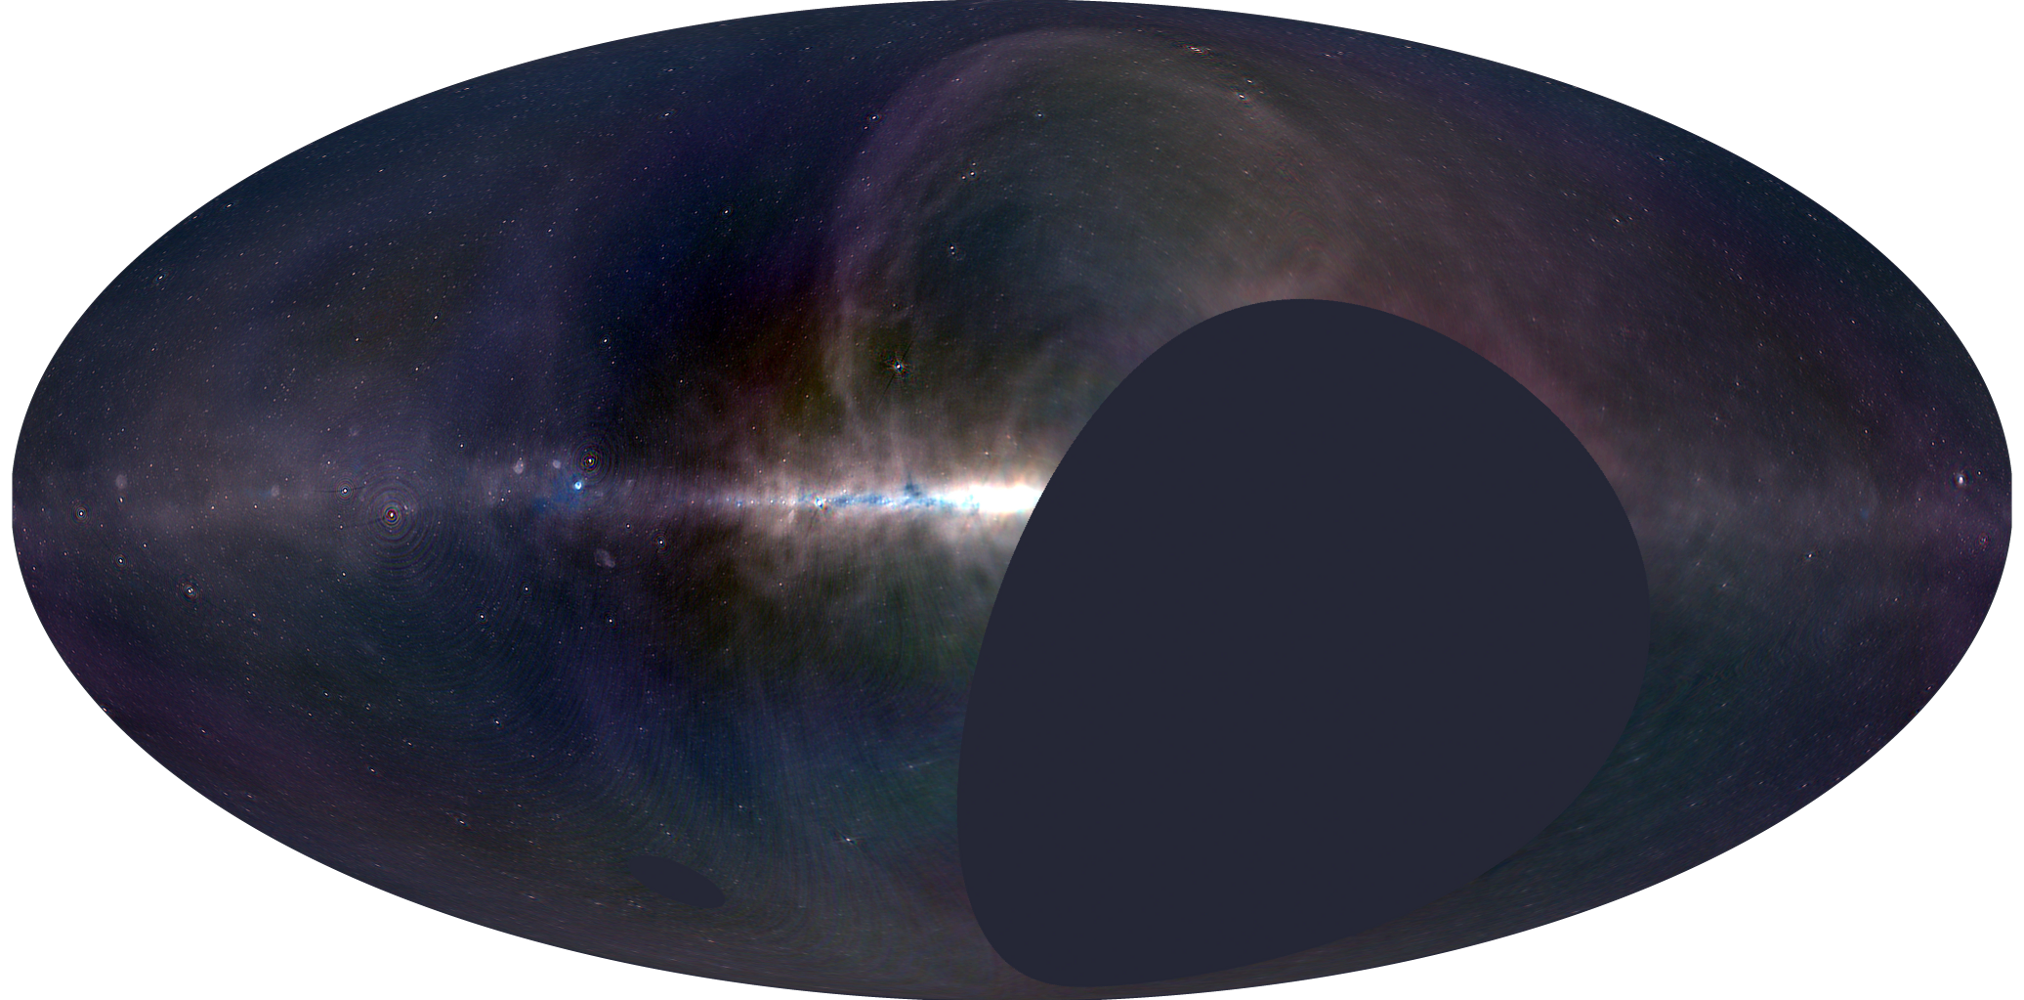
\includegraphics[width=\columnwidth, draft]{maps/rgb-map} &
        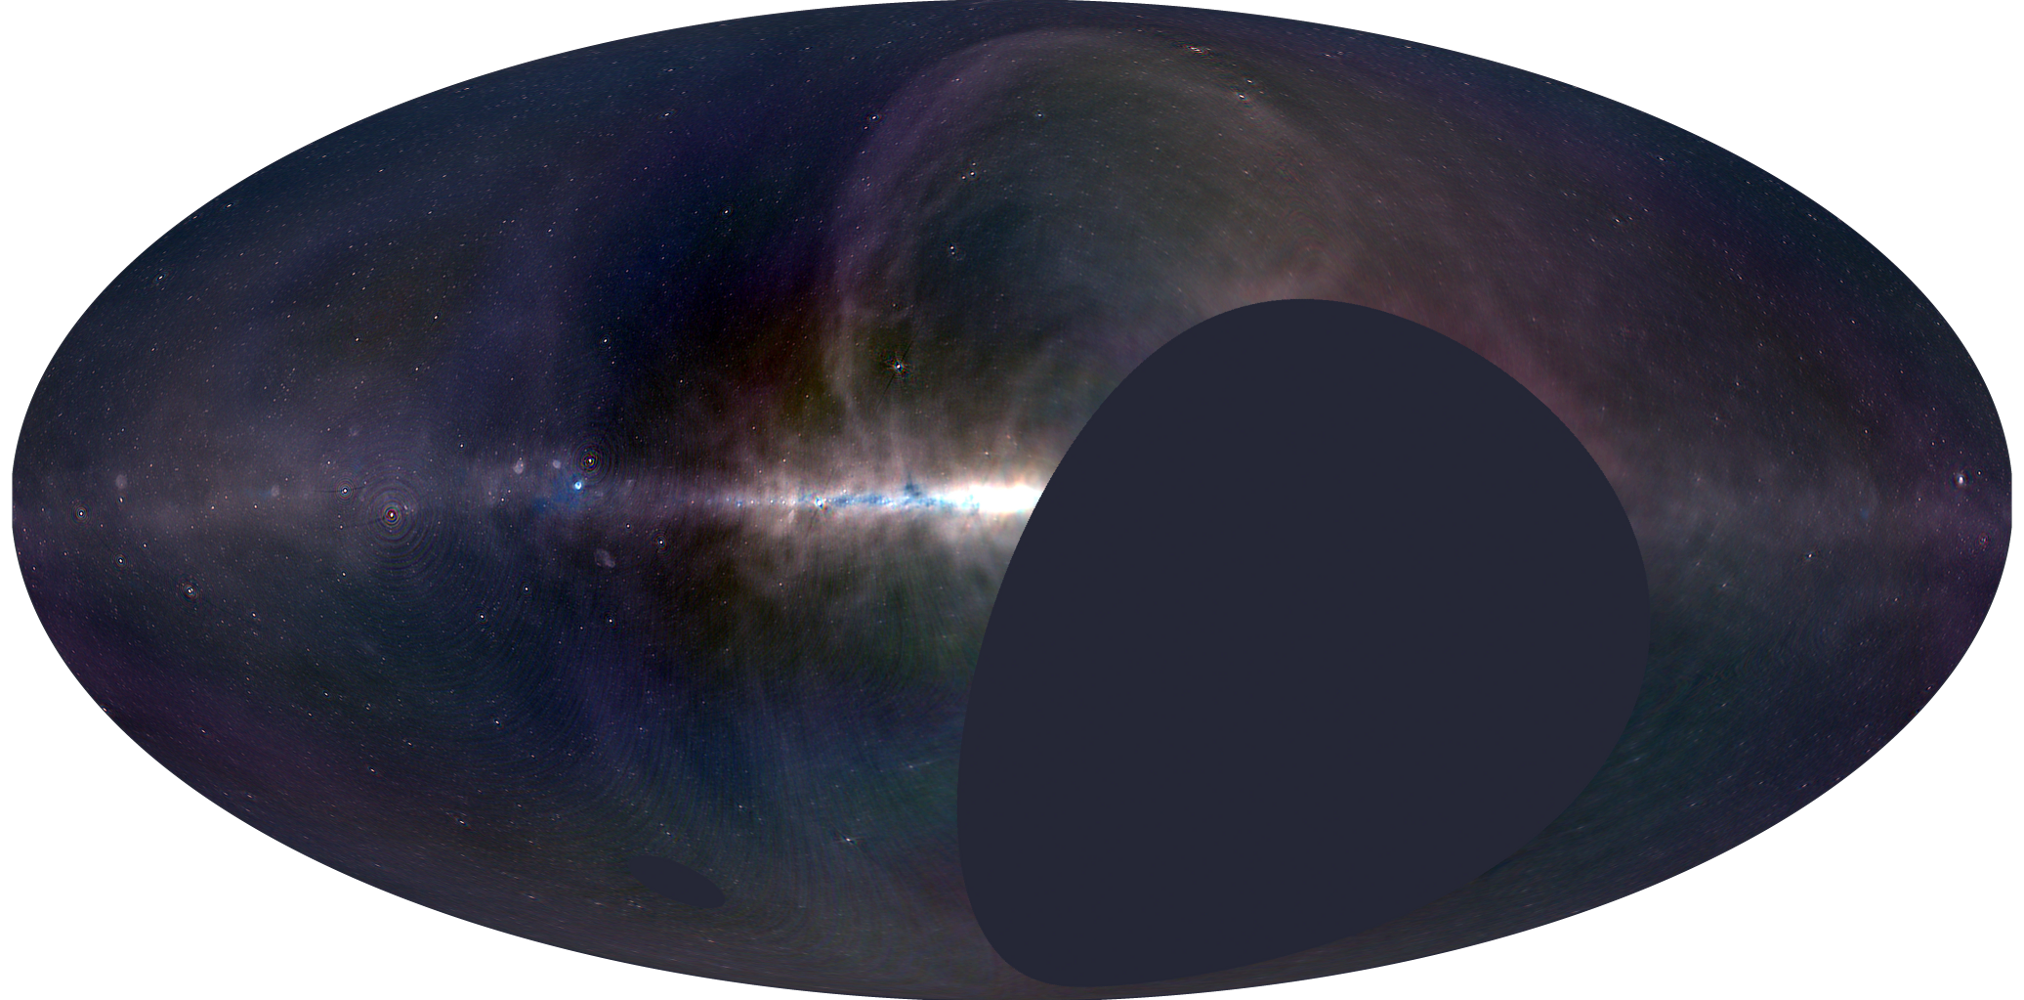
\includegraphics[width=\columnwidth, draft]{maps/rgb-map} \\
    \end{tabular}
    \caption{single channel maps}
\end{figure*}

\begin{figure*}[ht]
    \centering
    \begin{tabular}{cc}
        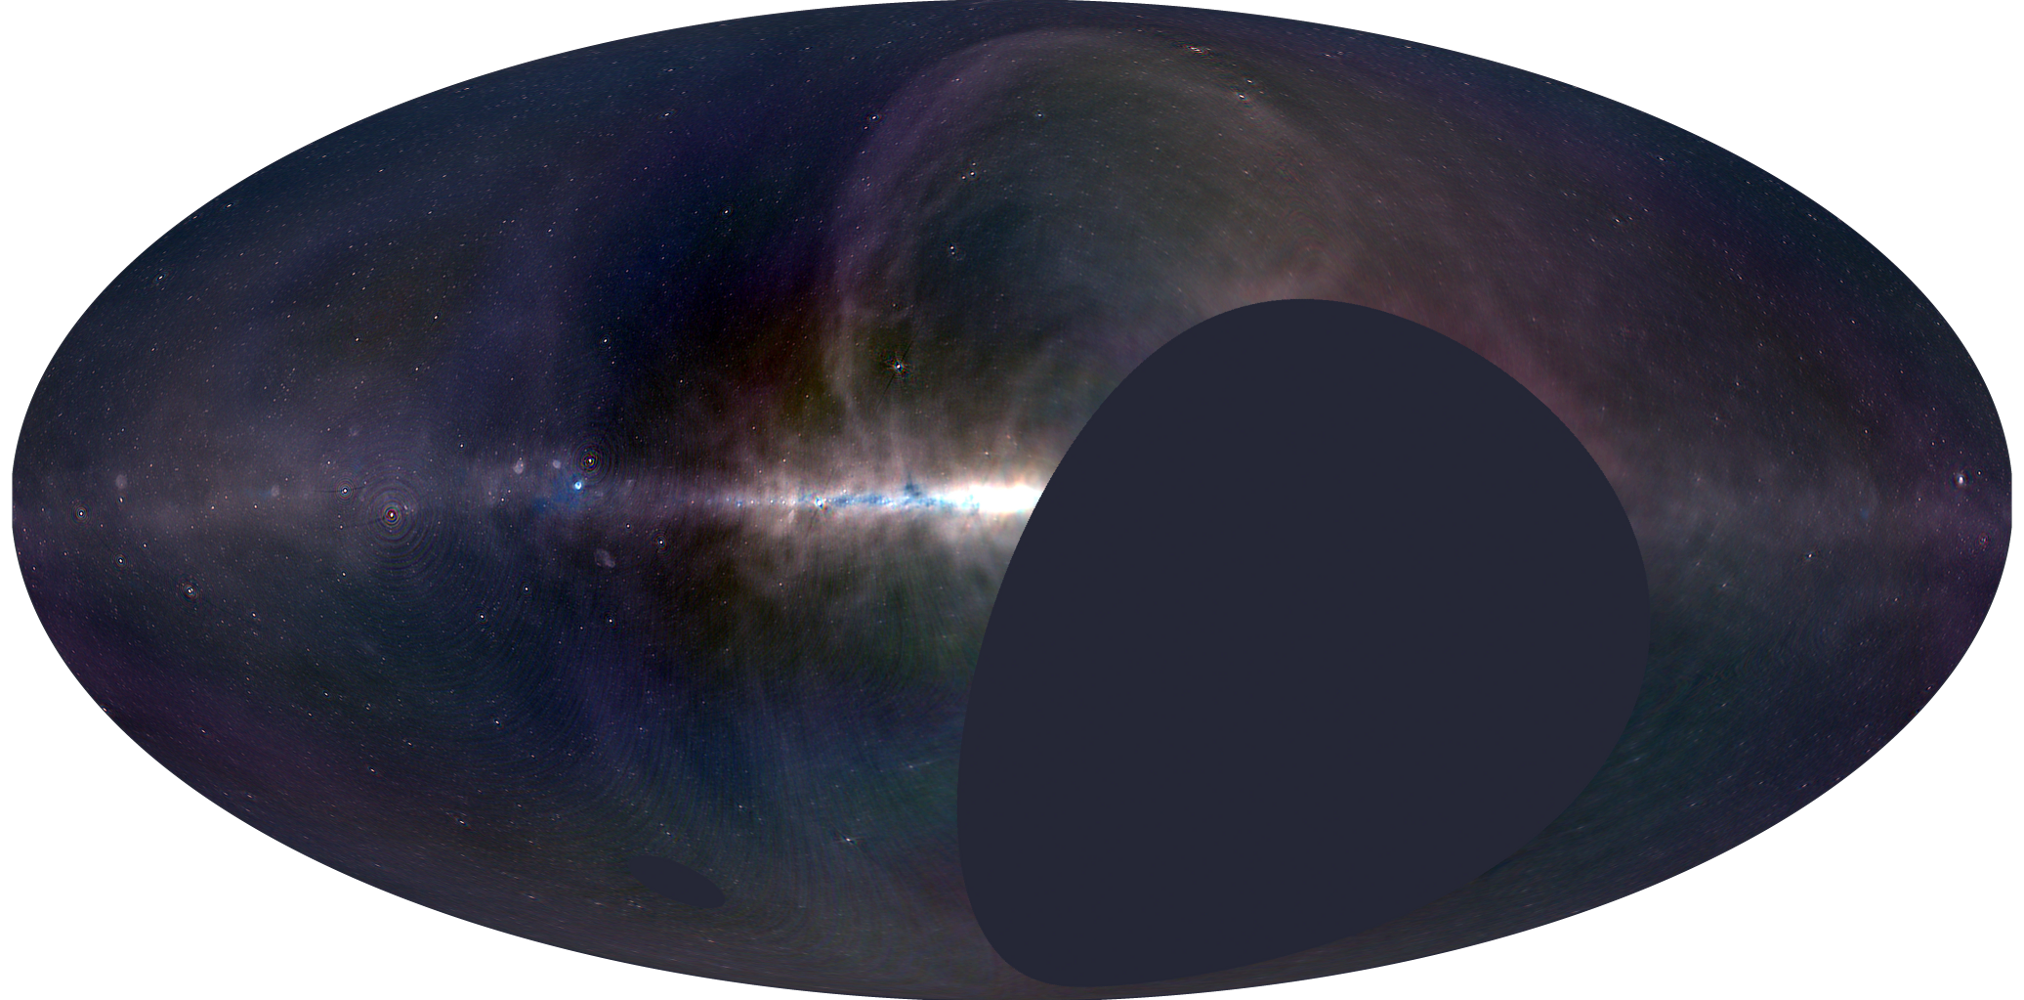
\includegraphics[width=\columnwidth, draft]{maps/rgb-map} &
        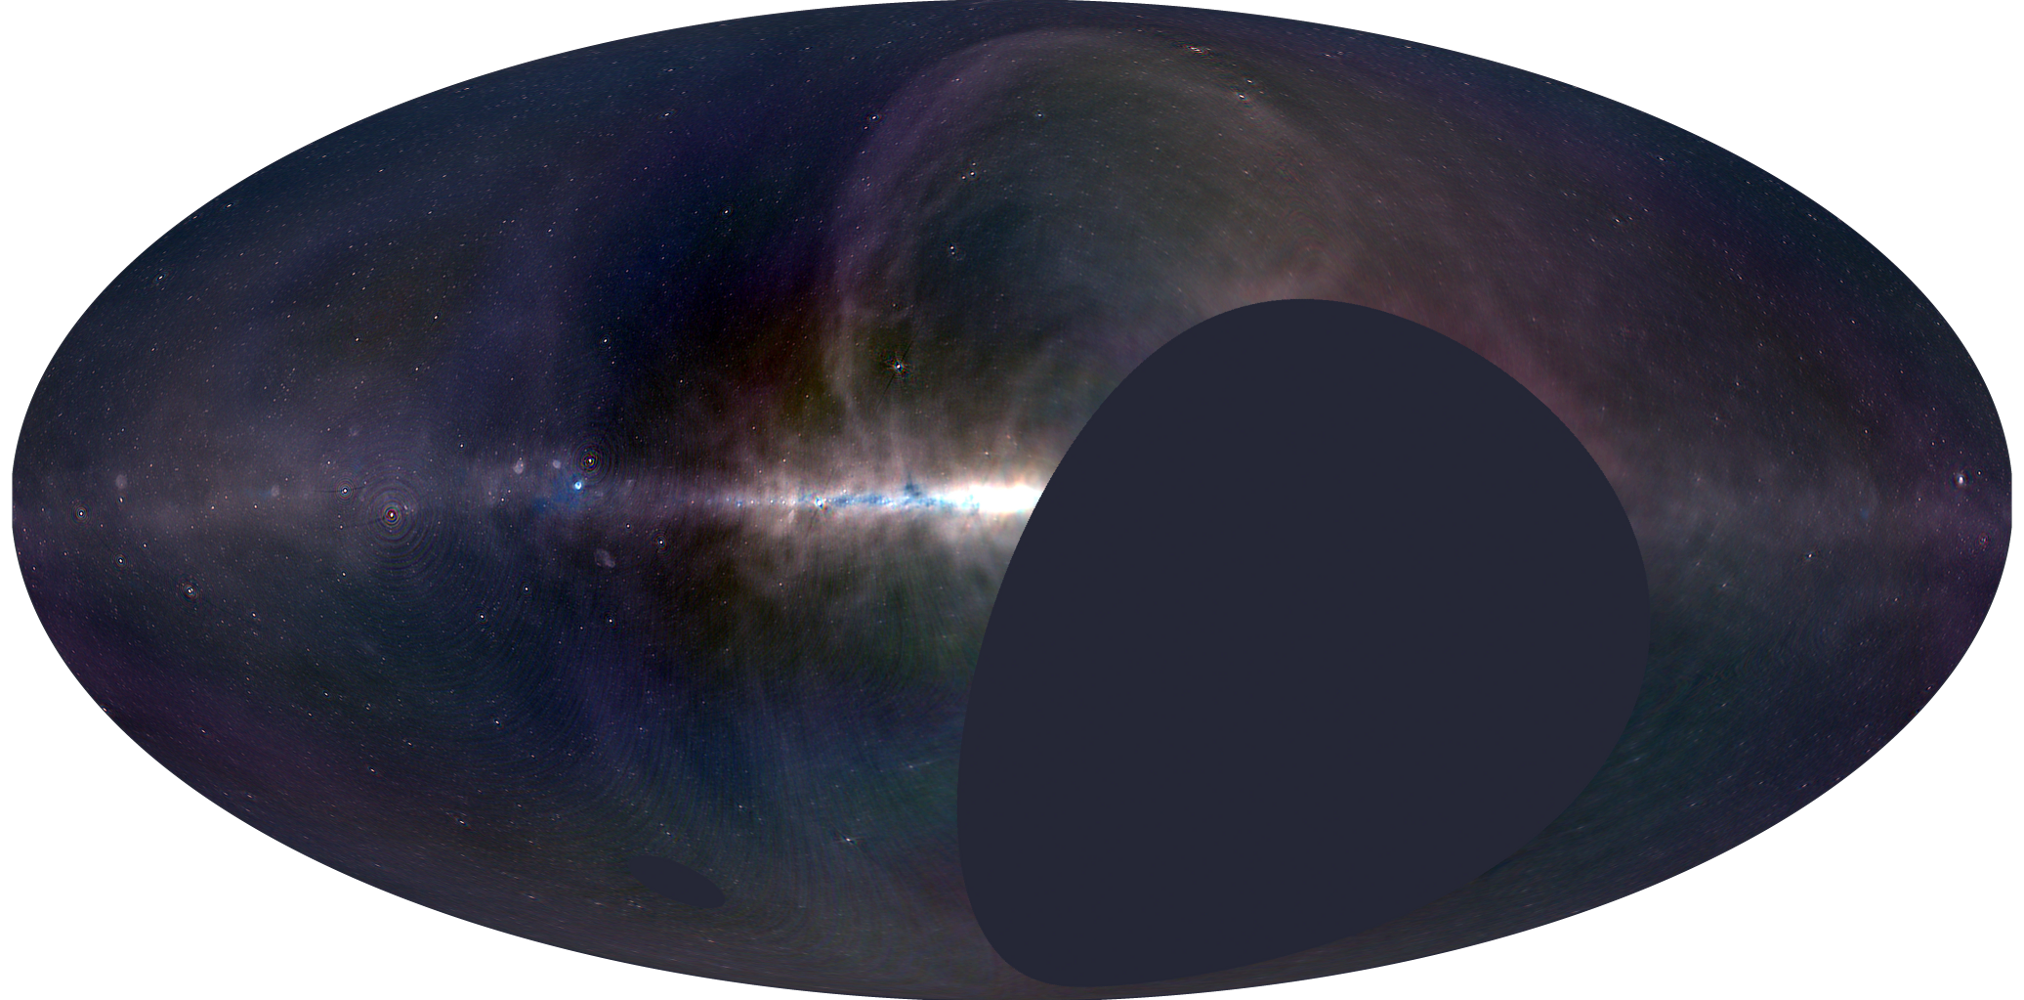
\includegraphics[width=\columnwidth, draft]{maps/rgb-map} \\
        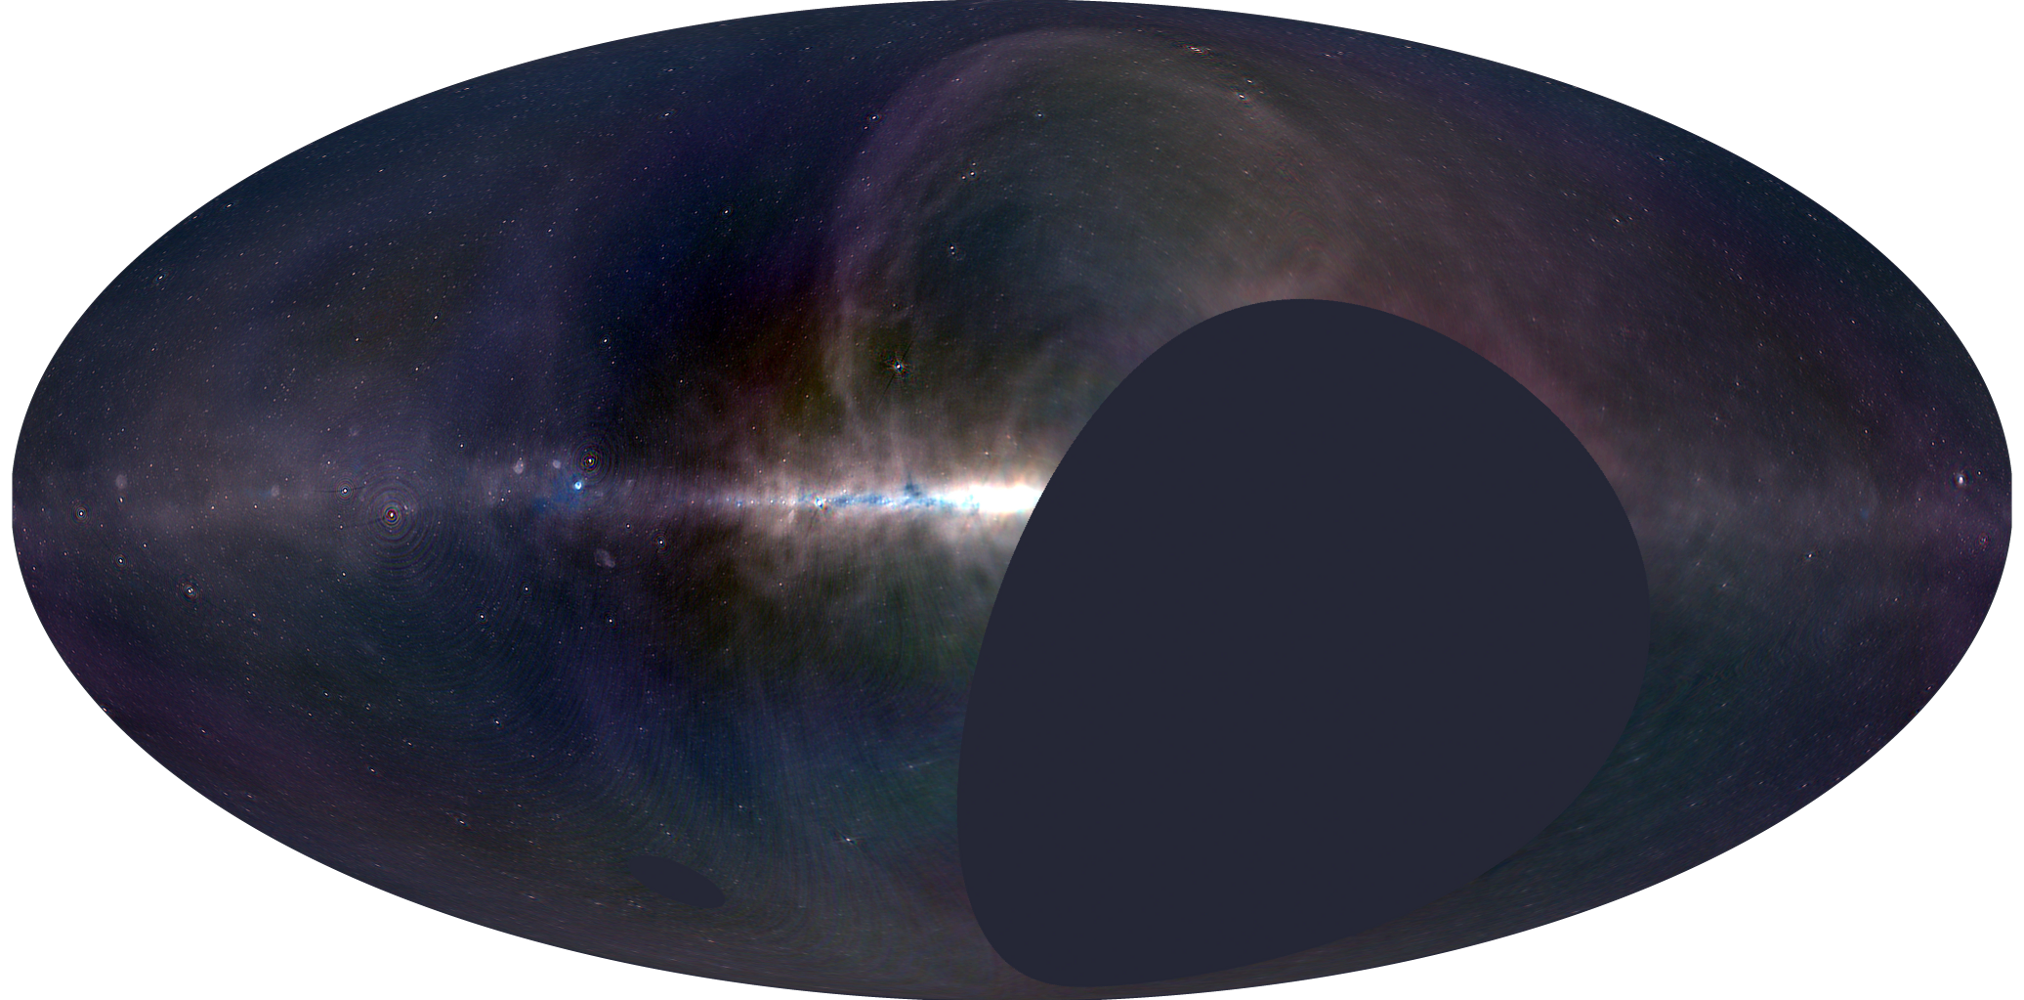
\includegraphics[width=\columnwidth, draft]{maps/rgb-map} &
        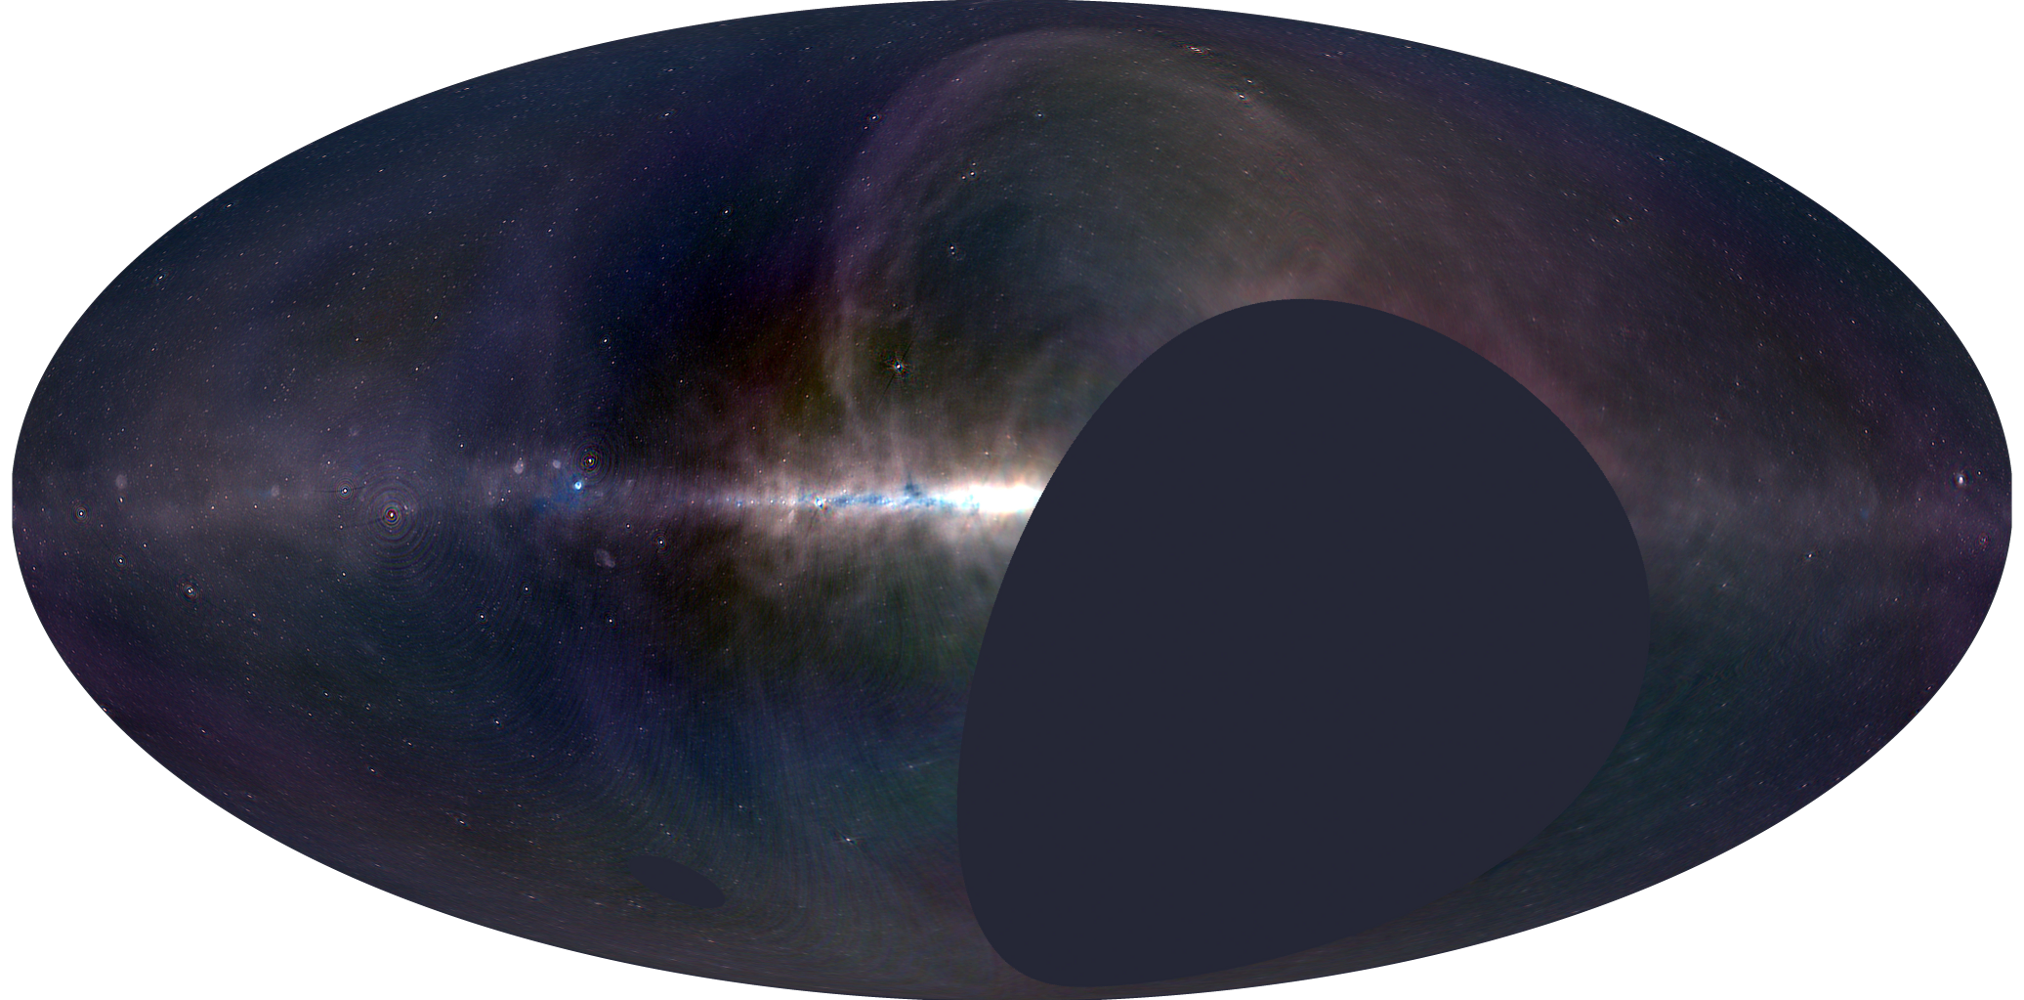
\includegraphics[width=\columnwidth, draft]{maps/rgb-map} \\
        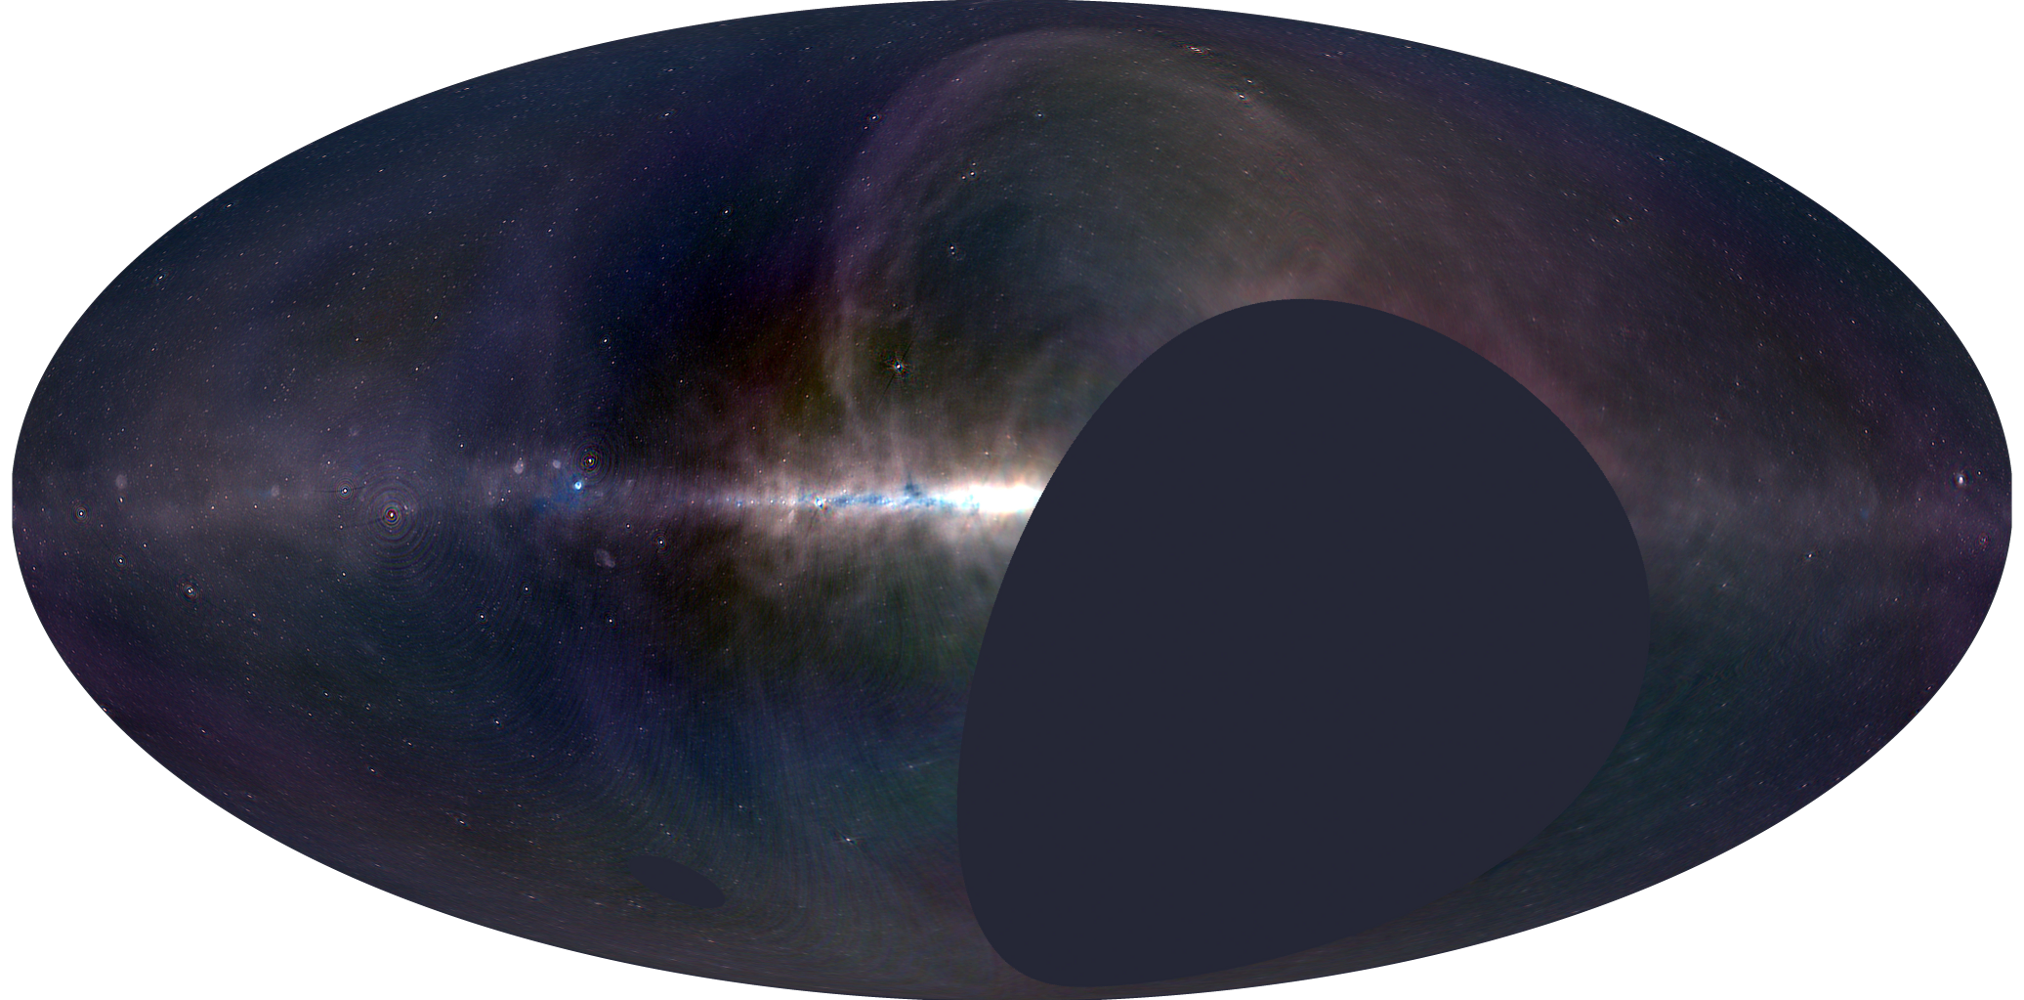
\includegraphics[width=\columnwidth, draft]{maps/rgb-map} &
        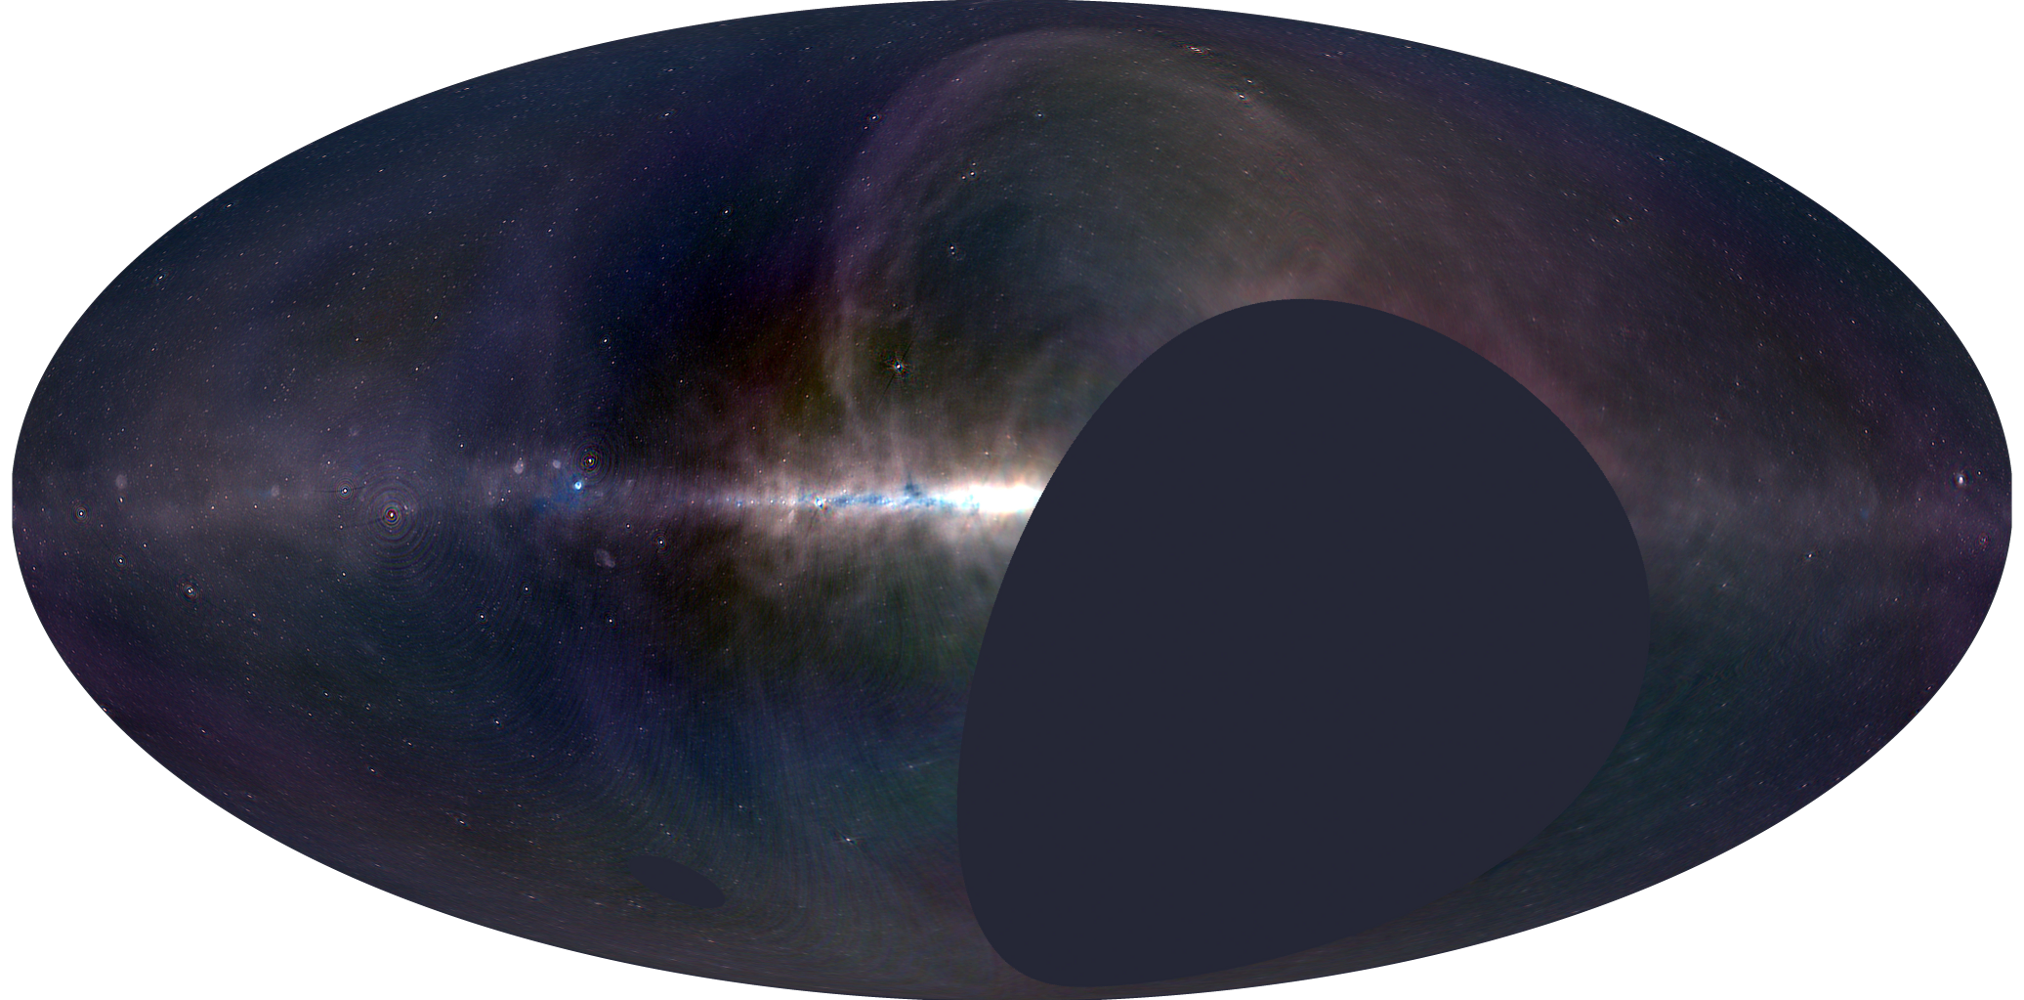
\includegraphics[width=\columnwidth, draft]{maps/rgb-map} \\
        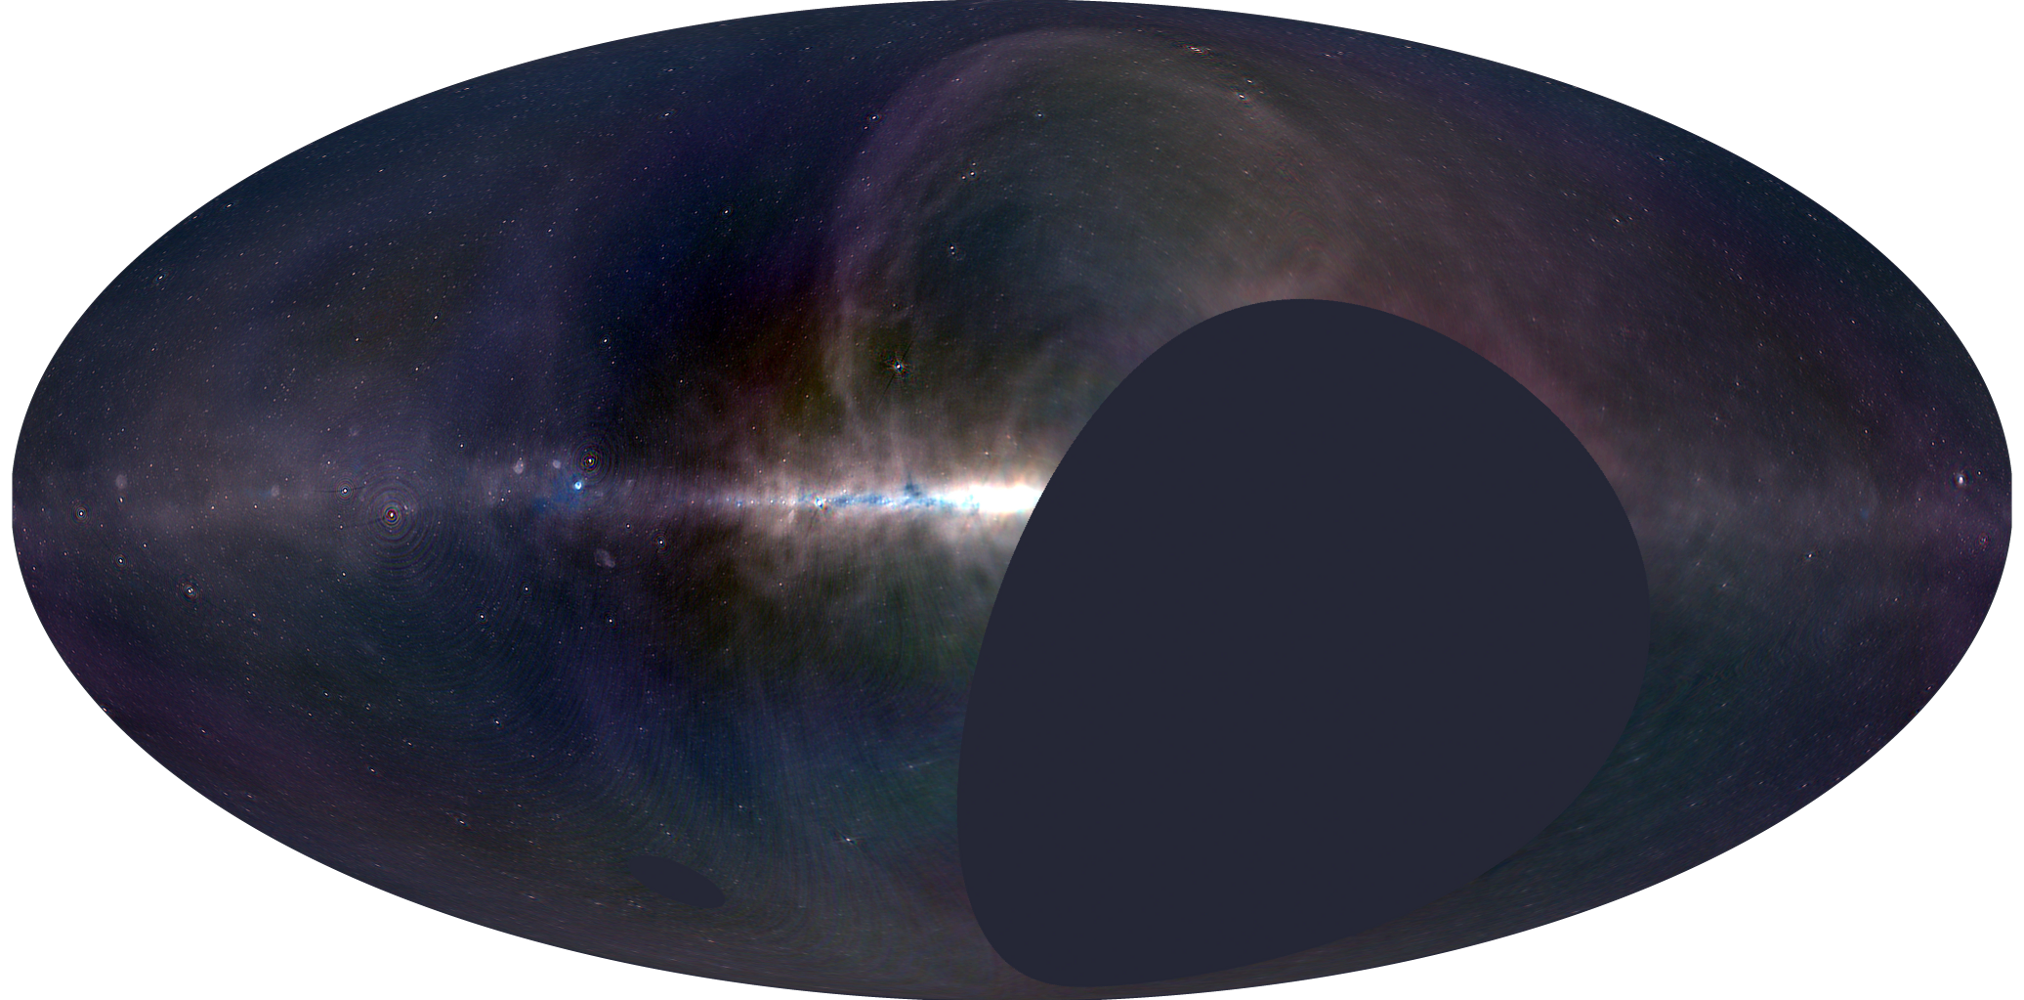
\includegraphics[width=\columnwidth, draft]{maps/rgb-map} &
        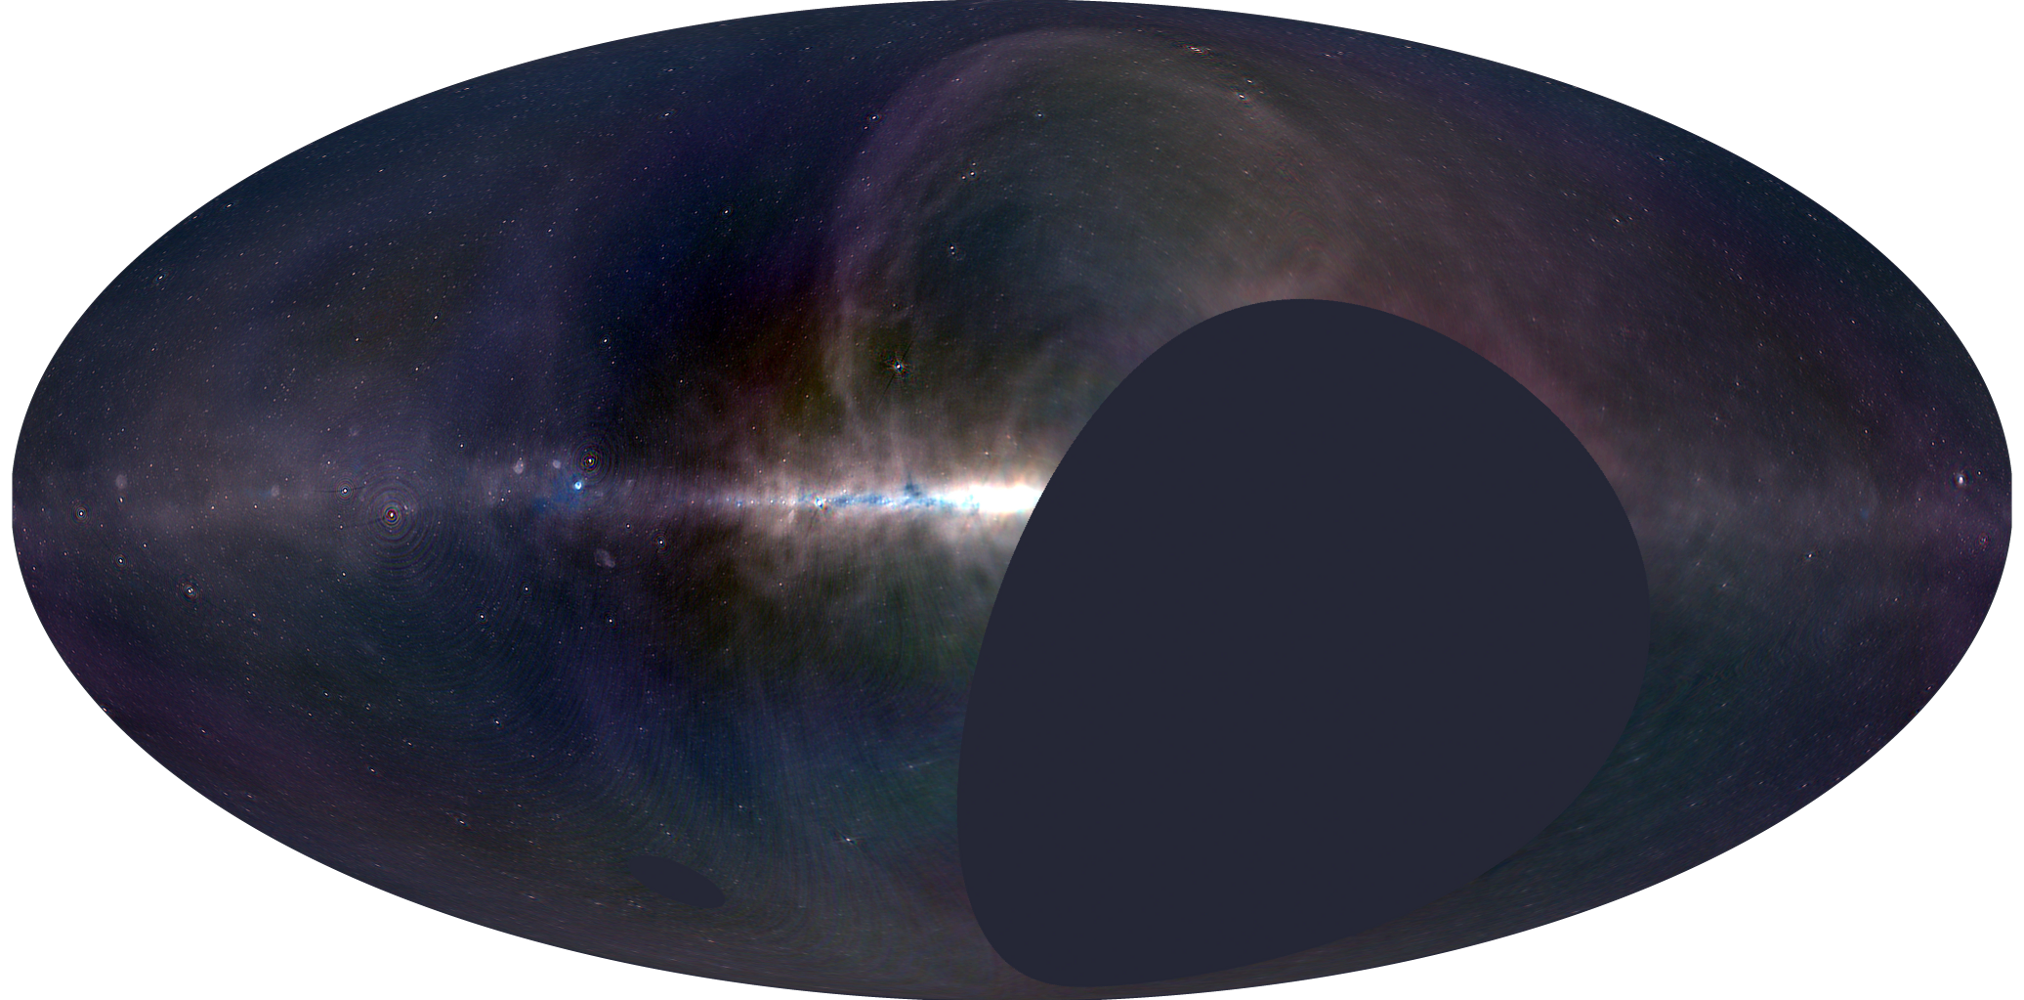
\includegraphics[width=\columnwidth, draft]{maps/rgb-map} \\
    \end{tabular}
    \caption{jackknifed error maps}
\end{figure*}

\begin{table}[ht]
    \centering
    \begin{tabular}{ccc}
        \# & $\nu$ / MHz & $\Delta\nu$ / MHz \\ \hline
        1 & 36.528 & 0.024 \\
        2 & 41.760 & 0.024 \\
        3 & 46.992 & 0.024 \\
        4 & 52.224 & 0.024 \\
        5 & 57.456 & 0.024 \\
        6 & 62.688 & 0.024 \\
        7 & 67.920 & 0.024 \\
        8 & 73.152 & 0.024 \\
    \end{tabular}
    \caption{Summary of the produced maps}
\end{table}

\subsection{Error Maps}


\todo{Cite Abhilash, Eastwood 2016}

\section{Discussion}

\bibliographystyle{apj}
\bibliography{paper}

\end{document}

